\chapter*{ESSEC-II 2018 : le corrigé}
  
%

\noindent
On s'intéresse à l'évolution d'une population de petits organismes 
(typiquement des insectes) pendant une \og saison \fg{} reproductrice 
de durée maximale $T$ où $T \in \N^*$. Les insectes sont supposés vivre 
une unité de temps, au bout de laquelle ils meurent en pondant un 
certain nombre d'{\oe}ufs. Au moment du dépôt d'un {\oe}uf, un 
processus chimique, la diapause, est susceptible de se mettre en marche 
qui entraîne l'arrêt de maturation de l'{\oe}uf jusqu'à la saison 
suivante. Ainsi, à chaque $t$ de la saison, une génération d'insectes 
s'éteint, en déposant des {\oe}ufs. Immédiatement, une proportion 
$p(t)$ de ces {\oe}ufs se mettent en diapause. Les {\oe}ufs qui ne sont 
pas entrés en diapause éclosent avant la date $t+1$, donnant naissance 
à une nouvelle génération d'insectes, qui s'éteindra à la date $t+1$ en 
déposant des {\oe}ufs, etc. Comme, à la fin de la saison, tous les 
organismes vivants de la population meurent, hormis les {\oe}ufs qui 
sont en diapause, ce sont ces derniers qui seront à l'origine d'une 
nouvelle population qui éclora à la saison suivante. Il est donc 
fondamental pour la survie de la lignée que les organismes adoptent une 
stratégie maximisant le nombre d'{\oe}ufs en diapause accumulés jusqu'à 
la date où la saison s'achève.\\[.1cm]
Au cours du problème, on s'intéressera plus particulièrement au cas où 
la durée de la saison est une variable aléatoire $\tau$ pouvant prendre 
des valeurs entières entre $1$ et $T$. Pour $t\in \{1,2, \ldots, T\}$, 
l'événement $\Ev{\tau=t}$ signifiera donc que la saison s'arrête à la 
date $t$.\\[.1cm]
Toutes les variables aléatoires intervenant dans le problème sont 
définies sur un espace probabilisé $(\Omega, \A, \Prob)$. Pour toute 
variable aléatoire $Y$, on notera $\E(Y)$ son espérance lorsqu'elle 
existe.



\section*{Partie I - Modèle de population saisonnière}

\noindent
\begin{minipage}{20cm}
  Dans cette question, on définit l'évolution formelle du nombre 
  d'{\oe}ufs en diapause entre les dates $0$ et $T$.
\end{minipage}

\noindent
On note $D(t)=$ nombre d'{\oe}ufs en diapause à la date $t$. Les 
{\oe}ufs pondus à la date $t$ qui entrent en diapause sont 
comptabilisés à la date $t+1$.
\[
  \begin{array}{rcR{12cm}}
    N(t) &=& nombre moyen d'{\oe}ufs produits à la date $t$
    \nl
    p(t) &=& proportion des {\oe}ufs produits à la date $t$ qui entrent 
    en diapause
  \end{array}
\]
Par convention, la date $0$ d'une saison est celle où les insectes nés 
des {\oe}ufs en diapause de la saison précédente pondent $N(0)$ 
{\oe}ufs. On suppose pour simplifier :
\begin{noliste}{$-$}
  \item que $N(0)$ est un entier naturel non nul.
  \item que tous les {\oe}ufs issus de la saison précédente ont éclos 
  et donc que $D(0)=0$.
  \item que pour tout $t\in \{0,1, \ldots, T-1\}$, $0<p(t)\leq 1$
\end{noliste}
Enfin, on suppose qu'à chaque date $t$ de la saison, un individu 
produit en moyenne $\alpha$ {\oe}ufs ($\alpha$ étant un réel 
strictement positif). {\bf Par simplicité, on supposera que $\alpha$ 
reste constant pendant toute la saison.}

\begin{noliste}{1.}
  \setlength{\itemsep}{4mm}
  \item 
  \begin{noliste}{a)}
    \setlength{\itemsep}{2mm}
    \item Montrer que $D(t+1)=D(t) + p(t) \, N(t)$ pour tout entier $t$ 
    tel que $0 \leq t \leq T-1$.
    
    \begin{proof}~\\
      Soit $t\in \{0,\ldots, T-1\}$.\\
      Le nombre d'{\oe}ufs en diapause à l'instant $(t+1)$, $D(t+1)$, 
      est la somme :
      \begin{noliste}{$\stimes$}
	\item du nombre d'{\oe}ufs qui étaient déjà en diapause à 
	l'instant $t$ : $D(t)$,
	\item et du nombre d'{\oe}ufs pondus à l'instant $t$ entrant 
	tout de suite en diapause.\\
	Or le nombre d'{\oe}ufs pondus à l'instant $t$ est $N(t)$, et
	la proportion d'entre eux entrant en diapause est $p(t)$.\\
	Ainsi le nombre d'{\oe}ufs pondus à l'instant $t$ entrant 
	immédiatement en diapause est : $p(t) \, N(t)$.
      \end{noliste}
      \conc{On en déduit : $\forall t \in \{0,\ldots, T-1\}$, $D(t+1) = 
      D(t) + p(t) \, N(t)$.}~\\[-1cm]
    \end{proof}
    
    
    \newpage

    
    \item Montrer que $N(t+1)=\alpha (1-p(t)) \, N(t)$ pour tout entier 
    $t$ tel que $0 \leq t \leq T-1$.
    
    \begin{proof}~\\
      Soit $t\in \{0,\ldots, T-1\}$.\\
      À l'instant $t$, $N(t)$ {\oe}ufs sont pondus. Parmi ceux-ci :
      \begin{noliste}{$\stimes$}
	\item $p(t) \, N(t)$ entrent immédiatement en diapause,
	
	\item $(1-p(t)) \, N(t)$ n'entrent pas en diapause.
      \end{noliste}
      Seuls les {\oe}ufs qui ne sont pas entrés en diapause à l'instant 
      $t$ produisent des {\oe}ufs à l'instant $(t+1)$. Donc 
      $(1-p(t)) \, N(t)$ individus produisent des {\oe}ufs à l'instant 
      $(t+1)$.\\
      D'après l'énoncé, chaque individu produit $\alpha$ {\oe}ufs.\\
      Ainsi, le nombre d'{\oe}ufs produits à l'instant $(t+1)$ est 
      $\alpha \, (1-p(t)) \, N(t)$.
      \conc{On en déduit : $\forall t \in \{0, \ldots, T-1\}$, 
      $N(t+1) = \alpha \, (1-p(t)) \, N(t)$.}~\\[-1cm]
    \end{proof}
  \end{noliste}
  
  \item On suppose dans cette question que $\alpha \leq 1$.
  \begin{noliste}{a)}
    \setlength{\itemsep}{2mm}
    \item Montrer que pour tout entier $t$ tel que $0 \leq t \leq T-1$,
    $N(t+1) \leq N(t)$.
    
    \begin{proof}~\\
    Soit $t \in \{0, \ldots, T-1\}$.
      \begin{noliste}{$\sbullet$}
	\item D'après la question précédente : $N(t+1) = \alpha \, (1-
	p(t)) \, N(t)$.
	
	\item Or, dans cette question : $\alpha \leq 1$.
	
	\item De plus, d'après l'énoncé : $0 < p(t) \leq 1$. D'où : 
	$0 \leq 1-p(t) <1$.
      \end{noliste}
      On en déduit : $\alpha \, (1-p(t)) \leq 1$. Ainsi :
      \[
        \begin{array}{ccc}
          \alpha \, (1-p(t)) \, N(t) & \leq & N(t)
          \\
          \shortparallel
          \\
          N(t+1)
        \end{array}
      \]
      \conc{$\forall t \in \{0, \ldots, T-1\}$, $N(t+1) \leq 
      N(t)$}~\\[-1cm]
    \end{proof}

    
    \item Montrer que pour tout entier $t$ tel que $0 \leq t \leq T-1$ :
    \[
      D(t+1) + N(t+1) \ \leq \ D(t)+N(t)
    \]
    
    \begin{proof}~\\
      Soit $t\in \{0, \ldots, T-1\}$.\\
      D'après les questions \itbf{1.a)} et \itbf{1.b)} :
      \[
        D(t+1) + N(t+1) \ = \ \big(D(t) + p(t) \, N(t)\big) + 
        \alpha \, (1-p(t)) \, N(t)
      \]
      Or $\alpha \leq 1$. On obtient donc : $ \alpha \, (1-p(t)) \, 
      N(t) \leq (1-p(t)) \, N(t)$.\\
      Ainsi :
      \[
       \begin{array}{rcl}
        D(t+1) + N(t+1) & \leq & D(t) + p(t) \, N(t) + (1-p(t)) \, N(t)
        \\[.2cm]
        &=& D(t) + (\bcancel{p(t)} + 1 - \bcancel{p(t)}) \, N(t)
        \\[.2cm]
        &=& D(t) + N(t)
       \end{array}
      \]
      \conc{$\forall t \in \{0, \ldots, T-1\}$, $D(t+1) + N(t+1) \leq 
      D(t) + N(t)$.}~\\[-1cm]
    \end{proof}
    
    
    \newpage
   
    
    \item Montrer que pour tout entier $t$ tel que $0 \leq t \leq T$ :
    \[
      D(t) + N(t) \leq N(0)
    \]
    
    \begin{proof}~\\
      Démontrons par récurrence que pour tout $t \in \{0, \ldots, T\}$, 
      $\PP{t}$ \quad où \quad $\PP{t}$ : $ D(t) + N(t) \leq N(0)$.
      \begin{noliste}{\fitem}
	\item {\bf Initialisation} :\\
	$D(0) + N(0) \ = \ 0 + N(0) \ = \ N(0) \ \leq \ N(0)$.\\
	D'où $\PP{0}$.
	
	\item {\bf Hérédité} : Soit $t\in \{0, \ldots, T-1\}$.\\
	Supposons $\PP{t}$ et démontrons $\PP{t+1}$ (\ie $D(t+1) + 
	N(t+1) \leq N(0)$)
	\[
	  \begin{array}{rcl@{\qquad}>{\it}R{5cm}}
	    D(t+1) + N(t+1) & \leq & D(t) + N(t) & (d'après la question 
	    \itbf{2.b)})
	    \nl
	    \nl[-.2cm]
	    & \leq & N(0) & (par hypothèse de récurrence)
	  \end{array}
	\]
	D'où $\PP{t+1}$.
      \end{noliste}
      \conc{Par principe de récurrence : $\forall t \in \{0, \ldots, 
      T\}$, $D(t) + N(t) \leq N(0)$.}
      
      \begin{remarkL}{.99}
        On pouvait sans doute obtenir la quasi-totalité des points 
        alloués à cette question sans effectuer proprement la 
        récurrence. Cela donnerait la rédaction suivante.\\
        Soit $t\in \{0, \ldots, T-1\}$.
        \begin{noliste}{$\sbullet$}
	  \item D'après la question précédente : $D(t+1) + N(t+1) \leq 
	  D(t) + N(t)$.
	  
	  \item En appliquant cette inégalité à $t-1$, on obtient :
	  $D(t) + N(t) \leq D(t-1) + N(t-1)$.
	  
	  \item Si on itère ce procédé, on en déduit :
	  \[
	    D(t+1) + N(t+1) \ \leq \ D(t) + N(t) \ \leq \
	    D(t-1) + N(t-1) \ \leq \ \cdots \ \leq \ D(1) + N(1) \
	    \leq \ D(0) + N(0)
	  \]
	  
	  \item Or, d'après l'énoncé, $D(0)=N(0)$. D'où : $D(t)
	  + N(t) \leq N(0)$.
        \end{noliste}
      \end{remarkL}~\\[-1.4cm]
    \end{proof}

    
    \item Montrer que pour tout entier $t$ tel que $0 \leq t \leq T$, 
    $D(t) \leq N(0)$.
    
    \begin{proof}~\\
      Soit $t \in \{0, \ldots, T\}$.\\
      D'après la question précédente : $D(t) + N(t) \leq N(0)$.\\
      Or $N(t)$ est un entier naturel. En particulier : $N(t) \geq 0$.\\
      Ainsi : $D(t) \leq D(t) + N(t) \leq N(0)$.
      \conc{$\forall t \in \{0, \ldots, T\}$, $D(t) \leq N(0)$}~\\[-1cm]
    \end{proof}

    
    \item On suppose que $p(0)=1$.
    \begin{nonoliste}{(i)}
      \item Montrer que pour tout entier $t$ tel que $1 \leq t \leq T$, 
      $N(t)=0$.
      
      \begin{proof}~\\
        Démontrons pas récurrence que pour tout $t \in \{1, \ldots, 
	T\}$, $\PP{t}$ \quad où \quad $\PP{t}$ : $N(t)=0$.
        \begin{noliste}{\fitem}
	  \item {\bf Initialisation} :\\
	  D'après la question \itbf{1.b)} : $N(1) \ = \ \alpha \, 
	  (1-p(0)) \, N(0) \ = \ \alpha \, (\bcancel{1} - \bcancel{1})
	  \, N(0) \ = \ 0$.\\
	  D'où $\PP{1}$.
	  
	  
	  \newpage
	  
	  
	  \item {\bf Hérédité} : Soit $t \in \{1, \ldots, T-1\}$.\\
	  Supposons $\PP{t}$ et démontrons $\PP{t+1}$ (\ie $N(t+1)=0$).
	  \[
	    \begin{array}{rcl@{\qquad}>{\it}R{5cm}}
	      N(t+1) &=& \alpha \, (1-p(t)) \, N(t) 
	      & (d'après la question \itbf{1.b)})
	      \nl
	      \nl[-.2cm]
	      &=& \alpha \, (1-p(t)) \times 0 
	      & (par hypothèse de récurrence)
	      \nl
	      \nl[-.2cm]
	      &=& 0
	    \end{array}
	  \]
	  D'où $\PP{t+1}$.
        \end{noliste}
        \conc{Par principe de récurrence : $\forall t \in \{1, \ldots,
        T\}$, $N(t)=0$.}
        \begin{remarkL}{.99}
          Comme pour la question \itbf{2.c)}, 
	  on pouvait sans doute obtenir la quasi-totalité des points 
	  alloués à cette question sans effectuer proprement la 
	  récurrence. Cela donnerait la rédaction suivante.\\
	  Soit $t\in \{0, \ldots, T-1\}$.
	  \begin{noliste}{$\sbullet$}
	  \item D'après la question \itbf{1.b)} : $N(t+1) = 
	  \alpha \, (1-p(t)) \, N(t)$.
	  
	  \item En appliquant cette inégalité à $t-1$, on obtient :
	  $N(t) = \alpha \, (1-p(t-1)) \, N(t-1)$.
	  
	  \item Si on itère ce procédé, on en déduit :
	  \[
	   \begin{array}{rcl}
	    N(t+1) &=& \alpha \, (1-p(t)) \, N(t)
	    \\[.2cm]
	    &=&
	    \alpha^2 \, (1-p(t)) \, (1-p(t-1)) \, N(t-1) 
	    \\[.2cm]
	    &=& 
	    \cdots
	    \\[.2cm]
	    &=& \alpha^{t+1} \, (1-p(t)) \, (1-p(t-1)) \, 
	    \cdots \, (1-p(0)) \, N(0)
	   \end{array}
	  \]
	  
	  \item Or, d'après l'énoncé, $p(0)=1$. D'où : $1-p(0)=0$.\\
	  Ainsi : $N(t)=0$.
        \end{noliste}
        \end{remarkL}~\\[-1.4cm]
      \end{proof}

      
      \item Montrer que pour tout entier $t$ tel que $1 \leq t \leq T$,
      $D(t)=N(0)$.
      
      \begin{proof}~\\
        Démontrons par récurrence que pour tout $t \in \{1, \ldots, 
	T\}$, $\PP{t}$ \quad où \quad $\PP{t}$ : $D(t)=N(0)$.
        \begin{noliste}{\fitem}
	  \item {\bf Initialisation} :\\
	  D'après la question \itbf{1.a)} : $D(1) \ = \ D(0) + p(0) \, 
	  N(0) \ = \ 0 + 1 \times N(0) \ = \ N(0)$.\\
	  D'où $\PP{1}$.
	  
	  \item {\bf Hérédité} : Soit $t\in \{1, \ldots, T-1\}$.\\
	  Supposons $\PP{t}$ et démontrons $\PP{t+1}$ (\ie $D(t+1)
	  =N(0)$).
	  \[
	    \begin{array}{rcl@{\qquad}>{\it}R{5cm}}
	      D(t+1) &=& D(t) + p(t) \, N(t) 
	      & (d'après la question \itbf{1.a)})
	      \nl
	      \nl[-.2cm]
	      &=& D(t) + \bcancel{p(t) \times 0}
	      & (d'après la question \itbf{2.e)(ii)}, car $t\geq 1$)
	      \nl
	      \nl[-.2cm]
	      &=& N(0) & (par hypothèse de récurrence)
	    \end{array}
	  \]
	  D'où $\PP{t+1}$.
        \end{noliste}
        \conc{Par principe de récurrence : $\forall t \in \{1, \ldots, 
        T\}$, $D(t)=N(0)$.}~\\[-1cm]
      \end{proof}
      
      
      \newpage

      
      \item En déduire que si $\alpha \leq 1$, la meilleure stratégie 
      adaptée à la saison est que les $N(0)$ {\oe}ufs produits à la date
      $0$ entrent en diapause immédiatement.
      
      \begin{proof}~
        \begin{noliste}{$\sbullet$}
	  \item D'après l'énoncé, la stratégie optimale est la stratégie
	  qui maximise le nombre d'{\oe}ufs en diapause accumulés 
	  jusqu'à la date $T$ (date de fin de saison).
	  
	  \item Si $\alpha \leq 1$, d'après la question \itbf{2.d)} :
	  $D(t) \leq N(0)$.
	  
	  \item Or, d'après la question \itbf{2.e)(ii)}, si $p(0)=1$, 
	  alors $D(t)=N(0)$.\\
	  Le nombre d'{\oe}ufs en diapause à chaque instant $t\in \{1, 
	  \ldots, T\}$ est donc maximal si $p(0)=1$, c'est-à-dire si la 
	  proportion d'{\oe}ufs entrant en diapause à l'instant $0$
	  parmi les $N(0)$ vaut $1$.
        \end{noliste}
        \conc{Autrement dit, la stratégie optimale est que les $N(0)$
        {\oe}ufs produits à la date $0$\\
        entrent en diapause 
        immédiatement.}~\\[-1cm]
      \end{proof}

    \end{nonoliste}
  \end{noliste}
  
  \item {\bf On suppose désormais $\alpha >1$ jusqu'à la fin du 
  problème.}\\
  On introduit maintenant $\tau$ une variable aléatoire à valeurs dans 
  $\{1,2, \ldots, T\}$ qui représente la date où s'achève la saison. On 
  suppose que pour tout $t \in \{1,2, \ldots, T\}$, $\Prob(
  \Ev{\tau=t}) >0$.
  \begin{noliste}{a)}
    \setlength{\itemsep}{2mm}
    \item Montrer que pour tout $t\in \{1,2, \ldots, T\}$, $\Prob(
    \Ev{\tau \geq t}) >0$. On définit alors $H(t)= \Prob_{\Ev{\tau \geq 
    t}}(\Ev{\tau =t})$.
    
    \begin{proof}~\\
      Soit $t\in \{1, \ldots, T\}$.\\
      Tout d'abord : $\Ev{\tau =t} \subset \Ev{\tau \geq t}$.
      Donc : $\Prob(\Ev{\tau = t}) \leq \Prob(\Ev{\tau \geq t})$.\\
      Or, d'après l'énoncé : $\Prob(\Ev{\tau =t}) >0$. D'où :
      \[
        \Prob(\Ev{\tau \geq t}) \ \geq \ \Prob(\Ev{\tau =t}) \ > \ 0
      \]
      \conc{Ainsi : $\forall t \in \{1, \ldots, T\}$, $\Prob(\Ev{\tau 
      \geq t}) >0$.}~\\[-1cm]
    \end{proof}

    
    \item Montrer que : $H(t)= \dfrac{\Prob(\Ev{\tau=t})}{\Prob(\Ev{\tau
    \geq t})}$.
    
    \begin{proof}~\\
      Soit $t \in \{1, \ldots, T\}$.
      \[
        \begin{array}{rcl@{\qquad}>{\it}R{5cm}}
          H(t) &=& \Prob_{\Ev{\tau \geq t}}(\Ev{\tau = t})
          \\[.4cm]
          &=&
          \dfrac{\Prob(\Ev{\tau \geq t} \cap \Ev{\tau = t})}
          {\Prob(\Ev{\tau \geq t})}
          \\[.6cm]
          &=& \dfrac{\Prob(\Ev{\tau = t})}{\Prob(\Ev{\tau \geq t})}
          & (car $\Ev{\tau =t} \subset \Ev{\tau \geq t}$)
        \end{array}
      \]
      \conc{$\forall t \in \{1, \ldots, T\}$, $H(t) =
      \dfrac{\Prob(\Ev{\tau=t})}{\Prob(\Ev{\tau \geq t})}$}~\\[-1cm]
    \end{proof}

    
    \item Montrer que : $H(T)=1$.
    
    \begin{proof}~\\
      La \var $\tau$ est à valeurs dans $\{1, \ldots, T\}$. En 
      particulier, $\tau$ ne prend pas de valeurs strictement 
      supérieures à $T$.
      Donc : $\Ev{\tau \geq T} = \Ev{\tau = T}$.\\[.1cm]
      D'où : $H(t) \ = \ \dfrac{\Prob(\Ev{\tau = T})}
      {\Prob(\Ev{\tau \geq T})} \ = \ \dfrac{\bcancel{\Prob(
      \Ev{\tau =T})}}{\bcancel{\Prob(\Ev{\tau =T})}} \ = \ 1$.
      \conc{Ainsi : $H(T)=1$.}~\\[-1cm]
    \end{proof}
    
    
    \newpage

    
    \item Calculer $H(t)$ pour $t\in \{1,2, \ldots, T\}$ si $\tau$ 
    suit une loi uniforme sur $\{1,2, \ldots, T\}$.
    
    \begin{proof}~
      \begin{noliste}{$\sbullet$}
	\item Comme $\tau \suit \U{1}{T}$, alors :
	\begin{noliste}{$\stimes$}
	  \item $\tau(\Omega) = \llb 1, T\rrb$.
	  \item $\forall t \in \llb 1, T \rrb$, $\Prob(\Ev{\tau =t})
	  =\dfrac{1}{T}$.
	\end{noliste}
	
	\item Soit $t\in \llb 1, T\rrb$.
	\[
	  \Ev{\tau \geq t} \ = \ \dcup{k=t}{T} \Ev{\tau =k}
	\]
	De plus, les événements $\Ev{\tau=t}$, $\ldots$, $\Ev{\tau =
	T}$ sont incompatibles. Donc :
	\[
	  \Prob(\Ev{\tau \geq t}) \ = \ \Sum{k=t}{T} 
	  \Prob(\Ev{\tau =k}) \ = \ \Sum{k=t}{T} \dfrac{1}{T}
	  \ = \ \dfrac{T-t+1}{T}
	\]
	
	\item On en déduit :
	\[
	  H(t) \ = \ \dfrac{\Prob(\Ev{\tau =t})}{\Prob(\Ev{\tau \geq 
	  t})} \ = \ \dfrac{\frac{1}{\bcancel{T}}}{\frac{T-t+1}
	  {\bcancel{T}}} \ = \ \dfrac{1}{T-t+1}
	\]
      \end{noliste}
      \conc{$\forall t \in \{1, \ldots, T\}$, $H(t) = 
      \dfrac{1}{T-t+1}$}~\\[-1cm]
    \end{proof}

    
    \item 
    \begin{nonoliste}{(i)}
      \item Soient $T$ réels $\lambda_1$, $\lambda_2$, $\ldots$, 
      $\lambda_T$ tels que $0 < \lambda_1 < \lambda_2 < \cdots < 
      \lambda_T=1$. Par convention, on pose $\lambda_0=0$. Soient 
      $q_1=\lambda_1$, $q_2=\lambda_2-\lambda_1$, $\ldots$, 
      $q_T=\lambda_T - \lambda_{T-1}$.\\
      Montrer que $(q_i)_{1\leq i \leq T}$ définit une loi de 
      probabilité sur $\{1,2, \ldots, T\}$.
      
      \begin{proof}~
        \begin{noliste}{$\sbullet$}
	  \item Soit $i\in \llb 1, T\rrb$.\\
	  D'après l'énoncé : $\lambda_i > \lambda_{i-1}$. Donc 
	  $q_i = \lambda_i - \lambda_{i-1} >0$.
	  
	  \item De plus :
	  \[
	    \Sum{i=1}{T} q_i \ = \ \Sum{i=1}{T} (\lambda_i - 
	    \lambda_{i-1}) \ = \ \lambda_T - \lambda_0 \ = \ 1-0
	    \ = \ 1
	  \]
        \end{noliste}
        \conc{On en déduit que $(q_i)_{i \in \llb 1,T \rrb}$ 
        définit une loi de probabilité.}~\\[-1cm]
      \end{proof}

      
      \item Calculer $H(t)$ si $\tau$ suit la loi précédente.
      
      \begin{proof}~
        \begin{noliste}{$\sbullet$}
	  \item Si la \var $\tau$ suit la loi $(q_i)_{i \in \llb 1,T 
	  \rrb}$, alors :
	  \[
	    \forall t \in \llb 1,T \rrb, \ \Prob(\Ev{\tau =t}) = q_t
	  \]
	  
	  \item Soit $t\in \llb 1,T \rrb$.
	  Avec le même raisonnement qu'en question \itbf{3.d)} :
	  \[
	    \Prob(\Ev{\tau \geq t}) \ = \ \Sum{i=t}{T} 
	    \Prob(\Ev{\tau =i}) \ = \ \Sum{i=t}{T} q_i \ = \
	    \Sum{i=t}{T} (\lambda_i - \lambda_{i-1}) \ = \ 
	    \lambda_T - \lambda_{t-1}
	  \]
	  
	  \item Ainsi : $H(t) \ = \ \dfrac{\Prob(\Ev{\tau =t})}
	  {\Prob(\Ev{\tau \geq t})} \ = \ \dfrac{q_t}{\lambda_T - 
	  \lambda_{t-1}} \ = \ \dfrac{\lambda_t - \lambda_{t-1}}
	  {\lambda_T - \lambda_{t-1}}$.
        \end{noliste}
        \conc{$\forall t \in \llb 1,T \rrb$, $H(t) \ = \ \dfrac{q_t}
        {\lambda_T - \lambda_{t-1}} \ = \ \dfrac{\lambda_t - 
        \lambda_{t-1}}{\lambda_T - \lambda_{t-1}}$}~\\[-1cm]
      \end{proof}
      
      
     \newpage

      
      \item On suppose que $T\geq 2$ et de plus que pour tout entier 
      $n$ tel que $1 \leq n \leq T-1$, on a $\lambda_{n+1} - 
      \lambda_n \geq \lambda_n - \lambda_{n-1}$. Montrer que 
      $t \mapsto H(t)$ est croissante sur $\{1,2, \ldots, T\}$.
      
      \begin{proof}~\\
        Soit $t \in \llb 1, T-1 \rrb$. D'après la question 
	\itbf{3.e)(ii)} :
	\[
	  H(t+1) \geq H(t) \ \ \Leftrightarrow \ \ \dfrac{\lambda_{t+1}
	  -\lambda_t}{\lambda_T - \lambda_t} \geq 
	  \dfrac{\lambda_t - \lambda_{t-1}}{\lambda_T - \lambda_{t-1}}
	\]
	\begin{noliste}{$\sbullet$}
	  \item On sait déjà, d'après l'énoncé : $\lambda_{t+1} - 
	  \lambda_t \ \geq \ \lambda_t - \lambda_{t-1} \ \geq \ 0
	  \qquad (\star) $.
	  
	  \item De plus :
	  \[
	    \begin{array}{rcl@{\qquad}>{\it}R{5cm}}
	      \dfrac{1}{\lambda_T - \lambda_t} \geq 
	      \dfrac{1}{\lambda_T - \lambda_{t-1}}
	      & \Leftrightarrow & \lambda_T - \lambda_t \leq 
	      \lambda_T - \lambda_{t-1}
	      & (par stricte décroissance de la fonction inverse sur 
	      $]0,+\infty[$)
	      \nl
	      \nl[-.2cm]
	      & \Leftrightarrow & \lambda_{t-1} \leq \lambda_t
	    \end{array}
	  \]
	  La dernière inégalité est vraie. Donc, par équivalence, la 
	  première également. On a donc :
	  \[
	    \dfrac{1}{\lambda_T - \lambda_t} \ \geq \ 
	    \dfrac{1}{\lambda_T - \lambda_{t-1}} \ \geq \ 0
	  \]
	  
	  \item On multiplie cette inégalité et l'inégalité $(\star)$
	  membre à membre
	  (ce qui ne change pas leurs sens car les termes en présence
	  sont positifs). On obtient alors :
	  \[
	   \begin{array}{ccc}
	    \dfrac{\lambda_{t+1} - \lambda_t}{\lambda_T - \lambda_t} 
	    & \geq & 
	    \dfrac{\lambda_t - \lambda_{t-1}}{\lambda_T - \lambda_{t-1}}
	    \\
	    \shortparallel & & \shortparallel
	    \\
	    H(t+1) & & H(t)
	   \end{array}
	  \]
	\end{noliste}
	\conc{On en déduit que $t \mapsto H(t)$ est croissante sur 
	$\{1, \ldots, T\}$.}~\\[-1.2cm]
      \end{proof}
    \end{nonoliste}
  \end{noliste}
  
  \noindent
  {\bf On suppose désormais que $t \mapsto H(t)$ est croissante.} Le 
  but est maintenant de trouver une stratégie adéquate pour maximiser 
  la quantité $\E\big(\ln(D(\tau))\big)$. On va commencer par regarder 
  un exemple simple.
  
  \item On suppose ici que $T=2$, que $H$ est donnée par $H(1) =
  \dfrac{1}{2}$ et $H(2)=1$ et que $\alpha=4$.
  \begin{noliste}{a)}
    \setlength{\itemsep}{2mm}
    \item 
    \begin{nonoliste}{(i)}
      \item Déterminer $\Prob(\Ev{\tau=1})$.
      
      \begin{proof}~
        \begin{noliste}{$\sbullet$}
	  \item D'après la question \itbf{3.b)} : $H(1) = 
	  \dfrac{\Prob(\Ev{\tau =1})}{\Prob(\Ev{\tau \geq 1})}$. Donc :
	  \[
	    \Prob(\Ev{\tau =1}) \ = \ H(1) \, \Prob(\Ev{\tau \geq 1})
	    \ = \ \dfrac{1}{2} \, \Prob(\Ev{\tau \geq 1})
	  \]
	  
	  \item De plus, comme $T=2$ : $\tau (\Omega) = \{1,2\}$.\\
	  On en déduit : $\Ev{\tau \geq 1} = \Omega$. Donc :
	  \[
	    \Prob(\Ev{\tau \geq 1}) \ = \ \Prob(\Omega) \ = \ 1
	  \]
	  
	  \item Ainsi : $\Prob(\Ev{\tau =1}) \ = \ \dfrac{1}{2} \,
	  \Prob(\Ev{\tau \geq 1}) \ = \  \dfrac{1}{2} \times 1 \ = \
	  \dfrac{1}{2}$.
        \end{noliste}
        \conc{$\Prob(\Ev{\tau=1}) = \dfrac{1}{2}$}~\\[-1cm]
      \end{proof}
      
      
      \newpage

      
      \item Quelle est la loi de $\tau$ ?
      
      \begin{proof}~
        \begin{noliste}{$\sbullet$}
	  \item D'après les résultats de la question précédente : 
	  $\tau(\Omega) = \{1,2\}$ et $\Prob(\Ev{\tau=1}) = 
	  \dfrac{1}{2}$.
	  
	  \item La famille $(\Ev{\tau=1}, \Ev{\tau=2})$ est un 
	  système complet d'événements. Donc :
	  \[
	    \Prob(\Ev{\tau=2}) \ = \ 1-\Prob(\Ev{\tau =1}) \ = \ 1-
	    \dfrac{1}{2} \ = \ \dfrac{1}{2}
	  \]
	  
	  \item On reconnaît les caractéristiques d'une \var de loi 
	  uniforme sur $\{1,2\}$.
        \end{noliste}
        \conc{$\tau \suit \U{1}{2}$}~\\[-1.2cm]
      \end{proof}
    \end{nonoliste}
    
    \item Montrer que pour $D(1)$ et $N(1)$ donnés, $D(2)$ est maximum
    pour $p(1)=1$.
    
    \begin{proof}~
     \begin{noliste}{$\sbullet$}
      \item D'après la question \itbf{1.a)} : $D(2) = D(1) + p(1) \, 
      N(1)$.\\
      Donc l'entier $D(2)$ est maximal si $D(1)+p(1) \, N(1)$ l'est.
      
      \item Or, si $D(1)$ et $N(1)$ sont fixés, alors $D(1)+p(1) \, 
      N(1)$ est maximal si $p(1)$ l'est.
      
      \item De plus : $0< p(1) \leq 1$. Donc $p(1)$ est maximal 
      lorsque $p(1)=1$.
     \end{noliste}
     \conc{On en déduit que $D(2)$ est maximal lorsque 
     $p(1)=1$.}~\\[-1cm]
    \end{proof}

    
    \item On suppose $p(1)=1$. Montrer que :
    \[
      \E\big(\ln(D(\tau)\big) \ = \ \dfrac{1}{2} \, \ln\big((4-3 \, 
      p(0)) \, N(0)\big) + \dfrac{1}{2} \, \ln\big(p(0) \, N(0)\big)
    \]
    
    \begin{proof}~
      \begin{noliste}{$\sbullet$}
	\item La \var $\tau$ est une \var finie, donc la \var $\ln(
	D(\tau))$ l'est aussi.
	\conc{Ainsi, la \var $\ln(D(\tau))$ admet une espérance.}
	
	\item D'après le théorème de transfert :
	\[
	  \begin{array}{rcl}
	    \E\big(\ln(D(\tau))\big) &=& \ln(D(1)) \, \Prob(\Ev{\tau
	    =1}) + \ln(D(2)) \, \Prob(\Ev{\tau =2})
	    \\[.2cm]
	    &=& \dfrac{1}{2} \, \ln(D(1)) + \dfrac{1}{2} \, \ln(D(2))
	  \end{array}
	\]
	
	\item Or : $D(1) \ = \ D(0) + p(0) \, N(0) \ = \ p(0) \, N(0)$.
	
	\item De plus : 
	\[
	  \begin{array}{rcl}
	    D(2) &=& D(1) + p(1) \, N(1) \ = \ D(1) + N(1)
	    \\[.2cm]
	    &=& D(0) + p(0) \, N(0) + \alpha \, (1-p(0)) \, N(0)
	    \\[.2cm]
	    &=& p(0) \, N(0) + 4(1-p(0)) \, N(0)
	    \\[.2cm]
	    &=& (4-3 \, p(0)) \, N(0)
	  \end{array}
	\]
      \end{noliste}
      \conc{Finalement : $\E\big(\ln(D(\tau))\big) = \dfrac{1}{2} \,
      \ln\big(p(0) \, N(0)\big) + \dfrac{1}{2} \, \ln\big( (4-3 \, 
      p(0)) \, N(0) \big)$.}~\\[-1cm]
    \end{proof}
    
    
    \newpage

    
    \item Construire le tableau de variations sur $]0,1]$ de la 
    fonction $\varphi$ définie par :
    \[
      \varphi(x) \ = \ \dfrac{1}{2} \, \ln\big((4-3x) \, N(0)\big) 
      + \dfrac{1}{2} \, \ln\big(N(0) \, x\big)
    \]
    
    \begin{proof}~
      \begin{noliste}{$\sbullet$}
	\item La fonction $\varphi$ est dérivable sur $]0,1]$ en tant 
	que composée et somme de fonctions dérivables sur $]0,1]$. 
	En effet, $N(0) >0$, donc : $N(0) \, x \in \ ]0,N(0)]$ et 
	$(4-3x) \, N(0) \in [N(0), 4 \, N(0)[$.

	
	\item Soit $x \in \ ]0,1]$.
	\[
	  \begin{array}{rcl}
	    \varphi'(x) &=& \dfrac{1}{2} \, \dfrac{-3 \, \bcancel{N(0)}}
	    {(4-3x) \, \bcancel{N(0)}} + \dfrac{1}{2} \, 
	    \dfrac{\bcancel{N(0)}}{\bcancel{N(0)} \, x}
	    \\[.6cm]
	    &=& \dfrac{1}{2} \left( - \dfrac{3}{4-3x} + \dfrac{1}{x}
	    \right) \ = \ \dfrac{1}{2} \, \dfrac{-3x+4-3x}{x \, 
	    (4-3x)}
	    \\[.6cm]
	    &=& \dfrac{1}{2} \, \dfrac{4-6x}{x(4-3x)} \ = \ 
	    \dfrac{2-3x}{x(4-3x)}
	  \end{array}
	\]
	
	\item Comme $x \in \ ]0,1]$ : $x >0$ et $4-3x>0$. Donc :
	\[
	  \varphi'(x) \geq 0 \ \Leftrightarrow \ 2-3x \geq 0 \
	  \Leftrightarrow \ 2 \geq 3x \ \Leftrightarrow \ 
	  \dfrac{2}{3} \geq x
	\]
	On obtient le tableau de variations suivant :
	\begin{center}
        \begin{tikzpicture}[scale=0.8, transform shape]
          \tkzTabInit[lgt=4,espcl=3] 
          {$x$ /1, Signe de $\varphi'(x)$ /1, Variations de $\varphi$ 
	  /2} 
          {$0$, $\frac{2}{3}$, $1$}%
          \tkzTabLine{ , + ,z, - , } 
          \tkzTabVar{-/$-\infty$, +/$\varphi\big( \frac{2}{3}\big)$, 
	  -/$\ln(N(0))$}
        \end{tikzpicture}
      \end{center}
      
      Détaillons les éléments de ce tableau :
      \begin{noliste}{$\stimes$}
	\item Tout d'abord : $\dlim{x\to 0} \ln \big( (4-3x) \, N(0)
	\big) = \ln\big(4 \, N(0)\big)$. De plus : $\dlim{x\to 0}
	\ln\big( N(0) \, x \big) = -\infty$.\\[.1cm]
	D'où : $\dlim{x\to 0} \varphi(x)=-\infty$.
	
	\item Ensuite :
	\[
	  \varphi(1) \ = \ \dfrac{1}{2} \, \ln\big( (4-3\times 1) \,
	  N(0)\big) + \dfrac{1}{2} \, \ln(N(0) \times 1) \ = \
	  \dfrac{1}{2} \, \ln(N(0)) + \dfrac{1}{2} \, \ln(N(0))
	  \ = \ \ln(N(0))
	\]
      \end{noliste}
      \end{noliste}
      
      \begin{remark}
        On pouvait également essayer de simplifier l'expression de 
        $\varphi\big(\frac{2}{2}\big)$ :
        \[
          \begin{array}{rcl}
            \varphi\Big(\dfrac{2}{3}\Big) &=& \dfrac{1}{2} \, \ln\left( 
	    \left(4 - \bcancel{3} \times \dfrac{2}{\bcancel{3}}\right) 
	    \, N(0)\right) + \dfrac{1}{2} \, \ln\left(N(0) \times 
	    \dfrac{2}{3}\right)
	    \\[.6cm]
	    &=& \dfrac{1}{2} \, \ln(2 \, N(0)) + \dfrac{1}{2} \, \ln
	    \left( \dfrac{2}{3} \, N(0)\right) \ = \ \dfrac{1}{2}
	    \left(\ln(2 \, N(0)) + \ln\left(\dfrac{2}{3} \, N(0)\right)
	    \right)
	    \\[.6cm]
	    &=& \dfrac{1}{2} \left( \ln(2) + \ln(N(0)) + \ln(2) - \ln(3)
	    + \ln(N(0)) \right)
	    \\[.4cm]
	    &=& \ln(N(0)) + \ln(2) - \dfrac{1}{2} \, \ln(3)
	    \ = \ \ln\Big( \dfrac{2 \, N(0)}{\sqrt{3}}\Big)
          \end{array}
        \]
      \end{remark}~\\[-1.4cm]
    \end{proof}
    
    
    \newpage

    
    \item Déterminer $p^*(0)$ qui maximise $\E\big(\ln(D(\tau))\big)$.
    
    \begin{proof}~\\
      D'après les questions \itbf{4.c)} et \itbf{4.d)} : $\E\big(
      \ln(D(\tau))\big) = \varphi(p(0))$.\\
      Or, d'après la question \itbf{4.d)}, la fonction $\varphi$
      admet un unique maximum en $\dfrac{2}{3}$.
      \conc{Donc $\E\big(\ln(D(\tau))\big)$ est maximal pour 
      $p^*(0)= \dfrac{2}{3}$.}~\\[-1cm]
    \end{proof}
  \end{noliste}
\end{noliste}




\section*{Partie II - Transformation du problème}

\noindent
{\bf Par convention, on conviendra que si $h$ est une fonction 
numérique définie sur $\{0,1,2, \ldots, T\}$}, on a
\[
  \Sum{t=1}{0} h(t)=0
\]

\begin{noliste}{1.}
  \setlength{\itemsep}{4mm}
  \setcounter{enumi}{4}
  \item Montrer que pour tout $t \in \{0,1,2, \ldots, T\}$, $D(t) 
  +N(t) >0$.
  
  \begin{proof}~\\
    Démontrons par récurrence que pour tout $t\in \{0, \ldots, T\}$,
    $\PP{t}$ \quad où \quad $\PP{t}$ : $D(t)+N(t) >0$.
    \begin{noliste}{\fitem}
      \item {\bf Initialisation} :\\
      D'après l'énoncé, $N(0)$ est un entier naturel non nul. Donc :
      $D(0) + N(0) \ = \ 0 + N(0) \ > \ 0$.\\
      D'où $\PP{0}$.
      
      \item {\bf Hérédité} : Soit $t\in \{0, \ldots, T-1\}$.\\
      Supposons $\PP{t}$ et démontrons $\PP{t+1}$ (\ie $D(t+1) + 
      N(t+1) >0$).
      \[
        \begin{array}{rcl}
          D(t+1) + N(t+1) &=& D(t) + p(t) \, N(t) + \alpha \, 
          (1-p(t)) \, N(t)
          \\[.2cm]
          &=& D(t) + \big(p(t) + \alpha(1-p(t))\big) \, N(t)
          \\[.2cm]
          &=& D(t) + N(t) + \big(p(t) + \alpha (1-p(t)) -1\big) N(t)
          \\[.2cm]
          &=& D(t) + N(t) + (1-p(t))(\alpha -1) N(t)
        \end{array}
      \]
      Or :
      \begin{noliste}{$\stimes$}
	\item par hypothèse de récurrence : $D(t) + N(t) >0$,
	\item $1-p(t)\geq 0$, car $0<p(t) \leq 1$,
	\item $\alpha -1>0$, car $\alpha >1$,
	\item $N(t) \geq 0$, car $N(t)$ est un entier naturel.
      \end{noliste}
      On en déduit : $D(t+1) + N(t+1) >0$.\\
      D'où $\PP{t+1}$.
    \end{noliste}
    \conc{Par principe de récurrence : $\forall t \in \{0, \ldots, T\}$,
    $D(t)+N(t) >0$.}~\\[-1cm]
  \end{proof}
  
  
  \newpage

  
  On pose
  \[
    X(t) \ = \ \dfrac{D(t)}{D(t) + N(t)}
  \]  
  
  \item Montrer que pour tout $t\in \{0,1,2, \ldots, T-1\}$ :
  \[
    X(t+1) \ = \ \dfrac{p(t) + (1-p(t)) \, X(t)}{p(t) + \alpha \, 
    (1-p(t)) + (1-\alpha)(1-p(t)) \, X(t)}
  \]
  
  \begin{proof}~\\
    Soit $t\in \{0, \ldots, T-1\}$.
    \begin{noliste}{$\sbullet$}
      \item D'une part : $X(t+1) \ = \ \dfrac{D(t+1)}{D(t+1) + 
      N(t+1)} \ = \ \dfrac{D(t) + p(t) \, N(t)}{D(t) + p(t) \, N(t) 
      + \alpha \, (1-p(t)) \, N(t)}$.
      
      \item D'autre part :
      \[
        \begin{array}{cl}
          & \dfrac{p(t) + (1-p(t)) \, X(t)}{p(t) + \alpha \, 
          (1-p(t)) + (1-\alpha)(1-p(t)) X(t)}
          \\[.6cm]
          =& \dfrac{p(t) + (1-p(t)) \, \frac{D(t)}{D(t)+N(t)}}
          {p(t) + \alpha \, (1-p(t)) + (1-\alpha)(1-p(t)) 
          \frac{D(t)}{D(t)+N(t)}}
          \\[.8cm]
          =& \dfrac{\frac{p(t)(D(t)+N(t)) + (1-p(t))D(t)} 
	  {\bcancel{D(t)+N(t)}}}
          {\frac{(p(t) + \alpha(1-p(t))(D(t) +N(t)) + (1-\alpha) 
          (1-p(t))D(t)} 
	  {\bcancel{D(t)+N(t)}}}
	  \\[.8cm]
	  =& \dfrac{\bcancel{p(t) \, D(t)} + p(t) \, N(t) + D(t) 
	  - \bcancel{p(t) \, D(t)}}
	  {\big(p(t) + \alpha(1-p(t)) + (1-\alpha)(1-p(t))\big) D(t)
	  + p(t) \, N(t) + \alpha(1-p(t))N(t)}
        \end{array}
      \]
      Or :
      \[
        p(t) + \alpha(1-p(t)) + (1-\alpha)(1-p(t)) \ = \
        p(t)\big(\bcancel{1-\alpha} - \bcancel{(1-\alpha)}\big) +
        \bcancel{\alpha} + 1 - \bcancel{\alpha} \ = \ 1
      \]
      D'où :
      \[
        \dfrac{p(t) + (1-p(t)) \, X(t)}{p(t) + \alpha \, 
        (1-p(t)) + (1-\alpha)(1-p(t)) X(t)} \ = \
        \dfrac{D(t) + p(t) \, N(t)}{D(t) + p(t) \, N(t) 
        + \alpha \, (1-p(t)) \, N(t)}
        \ = \ X(t+1)
      \]
    \end{noliste}
    \conc{$\forall t \in \{0, \ldots, T-1\}$, $X(t+1) \ = \ \dfrac{p(t) 
    + (1-p(t)) \, X(t)}{p(t) + \alpha \, 
    (1-p(t)) + (1-\alpha)(1-p(t)) \, X(t)}$}~\\[-1cm]
  \end{proof}

  
  \item Soit $\xi \in [0,1]$ fixé. Pour $x \in [0,1]$, on pose :
  \[
    \psi_\xi(x) \ = \ \dfrac{x+ (1-x) \xi}{x + \alpha \, (1-x) + 
    (1- \alpha)(1-x)\xi}
  \]
  \begin{noliste}{a)}
    \setlength{\itemsep}{2mm}
    \item Montrer que $\psi_\xi$ est croissante sur $[0,1]$.
    
    \begin{proof}~
      \begin{noliste}{$\sbullet$}
	\item La fonction $\psi_\xi$ est dérivable sur $[0,1]$ en tant
	que quotient de fonctions dérivables sur $[0,1]$ dont le 
	dénominateur ne s'annule pas.\\
	Démontrons que le dénominateur ne s'annule effectivement pas.\\
	Soit $x \in [0,1]$.
	\[
	 \begin{array}{rcl}
	  x + \alpha(1-x) + (1-\alpha)(1-x) \, \xi &=&
	  \big(1-\alpha - (1-\alpha) \, \xi\big) \, x + \alpha 
	  +(1-\alpha) \, \xi 
	  \\[.2cm]
	  &=& 
	  (1-\alpha)(1-\xi) \, x + \alpha + (1-\alpha) \, \xi
	 \end{array}
	\]
	
	
	\newpage
	
	
	On en déduit :
	\[
	  \begin{array}{rcl@{\qquad}>{\it}R{4cm}}
	    x + \alpha(1-x) + (1-\alpha)(1-x) \, \xi = 0 
	    & \Leftrightarrow & 
	    (1-\alpha)(1-\xi) \, x + \alpha + (1-\alpha) \, \xi = 0
	    \\[.2cm]
	    & \Leftrightarrow & 
	    (1-\alpha)(1-\xi) \, x = -\big(\alpha + (1-\alpha) \, 
	    \xi\big)
	    \\[.2cm]
	    & \Leftrightarrow & 
	    x = - \dfrac{\alpha + (1-\alpha) \, \xi}{(1-\alpha)(1-\xi)}
	    = \dfrac{\alpha + (1-\alpha) \, \xi}{(\alpha-1)(1-\xi)}
	    & (si $\xi \neq 1$)
	  \end{array}
	\]
	Or :
	\[
	  \dfrac{\alpha + (1-\alpha) \, \xi}{(\alpha-1)(1-\xi)}
	  \ = \ \dfrac{1+(\alpha -1) + (1-\alpha) \, \xi}
	  {(\alpha-1)(1-\xi)} \ = \ 
	  \dfrac{1+(\alpha-1)(1-\xi)}{(\alpha-1)(1-\xi)}
	  \ > \ 1
	\]
	De plus $x\in [0,1]$. Donc $x \neq \dfrac{\alpha + (1-\alpha) \, 
	\xi}{(\alpha-1)(1-\xi)}$.\\
	Par équivalence, on en déduit bien :
	$x + \alpha(1-x) + (1-\alpha)(1-x) \, \xi \neq 0$, c'est-à-dire
	que le dénominateur de $\psi_\xi$ ne s'annule pas sur $[0,1]$
	si $\xi \neq 1$.\\[.1cm]
	Soit $x \in [0,1]$. Si $\xi = 1$ :
	\[
	  x + \alpha (1-x) + (1-\alpha)(1-x) \ = \
	  x + (1-x)\big(\bcancel{\alpha} +(1-\bcancel{\alpha})\big)
	  \ = \ \bcancel{x} +1- \bcancel{x} \ = \ 1
	\]
	Donc le dénominateur de $\psi_1$ est toujours non nul
	sur $[0,1]$.
	
	\begin{remark}
	  On détaille ici précisément la dérivabilité de $\psi_\xi$.
	  Les correcteurs n'en attendaient sans doute pas tant.
	\end{remark}

	
	\item Soit $x \in [0,1]$.
	\[
	  \psi_\xi(x) \ = \ 
	  \dfrac{x+ (1-x) \xi}{x + \alpha \, (1-x) + 
	  (1- \alpha)(1-x)\xi}
	  \ = \
	  \dfrac{(1-\xi) \, x + \xi}
	  {(1-\alpha)(1-\xi) \, x + \alpha + (1-\alpha) \, \xi}
	\]
	Donc :
	\[
	  \begin{array}{rcl}
	    \psi_\xi'(x) &=& 
	    \dfrac{(1-\xi)\big((1-\alpha)(1-\xi) \, x + \alpha 
	    + (1-\alpha) \, \xi\big) - \big((1-\xi) \, x + \xi\big)
	    (1-\alpha)(1-\xi)}
	    {\big((1-\alpha)(1-\xi) \, x + \alpha + (1-\alpha) \,
	    \xi\big)^2}
	    \\[.6cm]
	    &=& \dfrac{\bcancel{(1-\alpha)(1-\xi)^2 \, x} + 
	    (1-\xi)\big(\alpha + (1-\alpha) \, \xi\big) - 
	    \bcancel{(1-\alpha)(1-\xi)^2 \, x} - (1-\alpha)(1-\xi)
	    \, \xi}
	    {\big((1-\alpha)(1-\xi) \, x + \alpha + (1-\alpha) \,
	    \xi\big)^2}
	    \\[.6cm]
	    &=& \dfrac{(1-\xi)\big(\alpha + \bcancel{(1-\alpha) \, \xi}
	    - \bcancel{(1-\alpha) \, \xi}\big)}
	    {\big((1-\alpha)(1-\xi) \, x + \alpha + (1-\alpha) \,
	    \xi\big)^2}
	    \\[.6cm]
	    &=& \dfrac{\alpha (1-\xi)}
	    {\big((1-\alpha)(1-\xi) \, x + \alpha + (1-\alpha) \,
	    \xi\big)^2}
	  \end{array}
	\]
	Or $\alpha >1>0$ et $1-\xi \geq 0$ car $\xi \in [0,1]$. Donc :
	$\psi_\xi(x) \geq 0$.
	\conc{On en déduit que $\psi_\xi$ est croissante sur $[0,1]$.}
      \end{noliste}
      
      \begin{remark}
        On pouvait aussi démontrer la croissance de $\psi_\xi$ sur 
        $[0,1]$ en utilisant la définition de la croissance.
        \begin{noliste}{$\sbullet$}
	  \item Soit $x \in [0,1]$. On rappelle :
	  \[
	    \psi_\xi(x) \ = \ \dfrac{(1-\xi) \, x + \xi}
	    {(1-\alpha)(1-\xi) \, x + \alpha + (1-\alpha) \, \xi}
	  \]
	  
	  \item Comme $\xi \in [0,1]$, alors $1-\xi \geq 0$.\\
	  Donc la fonction affine $h_1 : x \mapsto (1-\xi) \, x + \xi$ 
	  est croissante sur $[0,1]$.
	  
	  \item Comme $\alpha >1$, alors $1-\alpha <0$.\\
	  Donc la fonction affine $h_2 : x \mapsto (1-\alpha)(1-\xi)
	  \, x + \alpha + (1-\alpha) \, \xi$ est décroissante sur 
	  l'intervalle $[0,1]$.\\
	  On démontre de plus : 
	  \[
	    \forall x \in [0,1], \ h_2(x) =
	    (1-\alpha)(1-\xi) \, x + \alpha + (1-\alpha) \, \xi
	    >0
	  \]
	  {\it (La démonstration est similaire à celle de \og 
	  $(1-\alpha)(1-\xi) \, x + \alpha + (1-\alpha) \, \xi \neq 
	  0$ \fg{})}
	  
	  \item Soit $(x,y) \in [0,1]^2$ tel que $x \leq y$. On obtient
	  alors :
	  \begin{noliste}{$\stimes$}
	    \item par croissance de $h_1$ sur $[0,1]$ :
	    $h_1(x) \leq h_2(x)$.
	    
	    \item par décroissance de $h_2$ sur $[0,1]$ : 
	    $h_2(x) \geq h_2(y)$.
	  \end{noliste}
	  De plus : $h_2(x) \geq h_2(y) >0$.\\
	  Donc, par décroissance de la fonction inverse sur 
	  $[0,+\infty[$ : $\dfrac{1}{h_2(x)} \leq 
	  \dfrac{1}{h_2(y)}$.\\[.1cm]
	  On en déduit :
	  \[
	    \begin{array}{ccc}
	      \dfrac{h_1(x)}{h_2(x)} & \leq & \dfrac{h_1(y)}{h_2(y)}
	      \\
	      \shortparallel & & \shortparallel
	      \\
	      \psi_\xi(x) & & \psi_\xi(y)
	    \end{array}
	  \]
	  {\it (On conserve le sens de l'inégalité tous les réels 
	  en présence sont positifs)}\\
	  Ainsi, on a bien démontré que la fonction $\psi_\xi$ est 
	  croissante sur $[0,1]$.
        \end{noliste}
      \end{remark}~\\[-1.4cm]
    \end{proof}

    
    \item Calculer $\psi_\xi(1)$.
    
    \begin{proof}~\\
      On applique la définition de $\psi_\xi$ :
      \[
        \psi_\xi(1) \ = \ \dfrac{1+(\bcancel{1} - \bcancel{1}) \, \xi}
        {1+ \alpha(\bcancel{1}-\bcancel{1}) + (1-\alpha)
        (\bcancel{1}-\bcancel{1}) \, \xi} \ = \ \dfrac{1}{1} \ = \ 1
      \]
      \conc{$\psi_\xi(1) = 1$}~\\[-1cm]
    \end{proof}

    
    \item 
    \begin{nonoliste}{(i)}
      \item Calculer $\psi_\xi(0)$. On pose désormais
      $
        A(\xi) \ = \ \psi_\xi(0)
      $
      
      \begin{proof}~\\
        On calcule :
        \[
          \psi_\xi(0) \ = \ \dfrac{0 + (1-0) \, \xi}{0 + \alpha
          (1-0) + (1-\alpha)(1-0) \, \xi} \ = \ 
          \dfrac{\xi}{\alpha + (1-\alpha) \, \xi}
        \]
        \conc{$A(\xi) \ = \ \psi_\xi(0) \ = \ 
        \dfrac{\xi}{\alpha + (1-\alpha) \, \xi}$}~\\[-1cm]
      \end{proof}
      
      
      \newpage

      
      \item Montrer que pour tout $t\in \{0,1,2, \ldots, T-1\}$, 
      $A(X(t)) \leq X(t+1) \leq 1$.
      
      \begin{proof}~\\
      Soit $t \in \{0, \ldots, T-1\}$.
        \begin{noliste}{$\sbullet$}
	  \item D'après la question \itbf{6.} : $X(t+1) = 
	  \psi_{X(t)}(p(t))$.
	  
	  \item D'après la question \itbf{7.a)}, la fonction 
	  $\psi_\xi$ est croissante sur $[0,1]$. Donc :
	  \[
	    \forall x \in [0,1], \ \psi_\xi(0) \leq \psi_\xi(x) 
	    \leq \psi_\xi(1)
	  \]
	  
	  \item Or d'après la question \itbf{7.b)}, $\psi_\xi(1)=1$, et
	  d'après la question \itbf{7.c)(i)}, $\psi_\xi(0)=A(\xi)$.
	  D'où :
	  \[
	    \forall x \in [0,1], \ A(\xi) \leq \psi_\xi(x) \leq 1
	  \]
	  
	  \item L'encadrement précédent est valable pour tout $x \in
	  [0,1]$ et pour tout $\xi \in [0,1]$.\\
	  On l'applique alors à $x=p(t) \in \ ]0,1]$ et $\xi = 
	  X(t) \in [0,1]$ (par définition de $X(t)$).\\
	  On obtient alors :
	  \[
	    A(X(t)) \ \leq \ X(t+1) \ \leq \ 1
	  \]
        \end{noliste}
        \conc{$\forall t \in \{0, \ldots, T-1\}$, $A(X(t)) \leq 
        X(t+1) \leq 1$}
        
        \begin{remark}
          On pouvait aussi utiliser la définition de $X$ pour montrer
          que : 
	  \[
	    \forall t \in \llb 0, T-1\rrb, \ X(t+1) \leq 1
          \]
          En effet, soit $t \in \llb 0, T-1\rrb$ :
          \begin{noliste}{$\stimes$}
            \item d'une part, $D(t+1) \geq 0$ et $N(t+1) \geq 0$. Donc 
            $D(t+1) \leq D(t+1) + N(t+1)$.
            \item d'autre part, $X(t+1) = \dfrac{D(t+1)}{D(t+1) + 
	    N(t+1)}$~\\
          \end{noliste}
          Finalement, on a bien : $X(t+1) \leq 1$.
        \end{remark}~\\[-1.4cm]
      \end{proof}

      
      \item Montrer que $\xi \mapsto A(\xi)$ est croissante sur $[0,1]$.
      
      \begin{proof}~
        \begin{noliste}{$\sbullet$}
	  \item On rappelle que, d'après la question \itbf{7.c)(i)} :
	  $\forall \xi \in [0,1]$, $A(\xi) = \dfrac{\xi}{\alpha +
	  (1-\alpha) \, \xi}$.
	  
	  \item La fonction $A$ est dérivable sur $[0,1]$ en tant que 
	  quotient de fonctions dérivables sur $[0,1]$ dont le 
	  dénominateur ne s'annule pas (même raisonnement qu'en question 
	  \itbf{7.a)}).
	  
	  \item Soit $\xi \in [0,1]$.
	  \[
	    A'(\xi) \ = \ \dfrac{\alpha + \bcancel{(1-\alpha) \, \xi}
	    - \bcancel{\xi(1-\alpha)}}{\big(\alpha + (1-\alpha) \,
	    \xi \big)^2} \ > \ 0
	  \]
	  \conc{On en déduit que la fonction $A$ est strictement 
	  croissante sur $[0,1]$.}~\\[-1.4cm]
        \end{noliste}
      \end{proof}
    \end{nonoliste}
  \end{noliste}
    
  \item Justifier l'égalité de variables aléatoires :
  \[
    D(\tau) \ = \ \dfrac{D(\tau)}{D(\tau-1)} \cdot \dfrac{D(\tau-1)}
    {D(\tau-2)} \cdot \cdots \cdot \dfrac{D(2)}{D(1)} \cdot 
    \dfrac{D(1)}{N(0)} \cdot N(0)
  \]
  
  \begin{proof}~
    \begin{noliste}{$\sbullet$}
      \item Par récurrence : $\forall t \in \{1, \ldots, T\}$, 
      $D(t) >0$.\\
      De plus : $N(0)>0$.
      
      
      \newpage
      
      
      \item Par simplification de fractions :
      \[
	\dfrac{D(\tau)}{\bcancel{D(\tau-1)}}
        \dfrac{\bcancel{D(\tau-1)}}{\bcancel{D(\tau-2)}} 
        \cdot \cdots \cdot 
	\dfrac{\bcancel{D(2)}}{\bcancel{D(1)}}
	\cdot \dfrac{\bcancel{D(1)}}{\bcancel{N(0)}} 
	\cdot \bcancel{N(0)}
	\ = \ D(\tau)
      \]
    \end{noliste}
    \conc{$D(\tau) = \dfrac{D(\tau)}{D(\tau-1)} \cdot 
    \dfrac{D(\tau-1)}{D(\tau-2)} \cdot \cdots \cdot \dfrac{D(2)}{D(1)}
    \cdot \dfrac{D(1)}{N(0)} \cdot N(0)$}
    
    \begin{remark}
      On peut démontrer proprement la propriété \og $\forall t \in 
      \{1, \ldots, T\}$, $D(t) >0$ par récurrence.\\
      Elle n'était sans doute pas nécessaire ici puisque l'intitulé de 
      la question commence par un \og justifier \fg{}.\\
      Détaillons cependant cette récurrence ci-après.\\
      Démontrons par récurrence que pour tout $t \in \{1, \ldots, T\}$,
      $\PP{t}$ : $D(t) >0$.
      \begin{noliste}{\fitem}
        \item {\bf Initialisation} :\\
        D'après la question \itbf{1.a)}, $D(1) = p(0) \, N(0)$.\\
        Or, d'après l'énoncé, $N(0)>0$ et $p(0)>0$. Donc $D(1) >0$.\\
        D'où $\PP{1}$.
        
        \item {\bf Hérédité} : Soit $t\in \{1, \ldots, T-1\}$.\\
        Supposons $\PP{t}$ et démontrons $\PP{t+1}$ (\ie $D(t+1)
        >0$).\\
        D'après la question \itbf{1.a)} : $D(t+1) = D(t) + p(t) \, 
        N(t)$.\\
        Or :
        \begin{noliste}{$\stimes$}
	  \item $D(t) >0$ par hypothèse de récurrence,
	  \item $p(t)>0$ d'après l'énoncé,
	  \item $N(t) \geq 0$ car $N(t)$ est un entier naturel.
        \end{noliste}
        Ainsi, on a bien : $D(t+1) >0$.\\
        D'où $\PP{t+1}$.
      \end{noliste}
      Par principe de récurrence : $\forall t \in \{1, \ldots, T\}$,
      $D(t) >0$.
    \end{remark}~\\[-1.4cm]
  \end{proof}
  
  
  
  \noindent
  On pose $\hat{R}(0) = \ln \left( \dfrac{D(1)}{N(0)}\right)$ et 
  $\hat{R}(t) = \ln \left( \dfrac{D(t+1)}{D(t)}\right)$ pour $1 \leq t 
  \leq T-1$.
  
  \item 
  \begin{noliste}{a)}
    \setlength{\itemsep}{2mm}
    \item Montrer que :
    \[
      \E\big(\ln(D(\tau))\big) \ = \ \ln(N(0)) + \E\left( \hat{R}(0)
      + \Sum{t=1}{\tau -1} \hat{R}(t)\right)
    \]
    
    \begin{proof}~
      \begin{noliste}{$\sbullet$}
	\item D'après la question précédente : 
	\[
	  \begin{array}{rcl}
	    \ln(D(\tau)) &=& \ln \left( \dfrac{D(\tau)}{D(\tau -1)}
	    \cdot \dfrac{D(\tau-1)}{D(\tau -2)} \cdot \cdots \cdot
	    \dfrac{D(2)}{D(1)} \cdot \dfrac{D(1)}{N(0)} \cdot N(0)
	    \right)
	    \\[.6cm]
	    &=& \ln\left( \dfrac{D(\tau)}{D(\tau -1)}\right) + 
	    \ln\left(\dfrac{D(\tau-1)}{D(\tau-2)}\right) +
	    \cdots + \ln\left(\dfrac{D(2)}{D(1)}\right) + 
	    \ln\left(\dfrac{D(1)}{N(0)}\right) + \ln(N(0))
	    \\[.6cm]
	    &=& \Sum{t=1}{\tau-1} \ln \left(\dfrac{D(t+1)}{D(t)}\right)
	    + \hat{R}(0) + \ln(N(0))
	    \\[.6cm]
	    &=& \Sum{t=1}{\tau-1} \hat{R}(t) + \hat{R}(0) + \ln(N(0))
	  \end{array}
	\]
	
	
	\newpage
	
	
	\item La \var $\ln(D(\tau))$ admet une espérance en tant que 
	variable aléatoire finie.\\
	Par linéarité de l'espérance :
	\[
	  \E\big(\ln(D(\tau))\big) \ = \ \E\left(\ln(N(0))\big) +
	  \hat{R}(0) + \Sum{t=1}{\tau-1} \hat{R}(t)\right) \ = \
	  \ln(N(0)) + \E\left(\hat{R}[0) + \Sum{t=1}{\tau-1}
	  \hat{R}(t)\right)
	\]
      \end{noliste}
      \conc{$\E\big(\ln(D(\tau))\big) \ = \ \ln(N(0)) + 
      \E\left(\hat{R}(0) + \Sum{t=1}{\tau-1} 
      \hat{R}(t)\right)$}~\\[-1cm]
    \end{proof}
    
    \item Montrer que : $\dfrac{D(1)}{N(0)} = \dfrac{\alpha \, X(1)}
    {1+(\alpha-1) \, X(1)}$.
    
    \begin{proof}~\\
      On calcule :
      \[
        \begin{array}{rcl@{\qquad}>{\it}R{2.5cm}}
          \dfrac{\alpha \, X(1)}{1+ (\alpha-1) X(1)} &=& 
          \dfrac{\alpha \, \frac{D(1)}{D(1)+N(1)}}{1+ (\alpha -1) \,
          \frac{D(1)}{D(1)+N(1)}}
          & (par définition de $X(1)$)
          \nl
          \nl[-.2cm]
          &=& \dfrac{\frac{\alpha \, D(1)}{\bcancel{D(1)+N(1)}}}
          {\frac{D(1)+N(1) + (\alpha-1) \, D(1)}
          {\bcancel{D(1)+N(1)}}}
          \ = \ \dfrac{\alpha \, D(1)}{\bcancel{D(1)} + N(1) + 
          (\alpha -\bcancel{1}) \, D(1)}
          \\[.6cm] 
          &=& \dfrac{\alpha \, D(1)}{N(1) + \alpha \, D(1)}
          \ = \ \dfrac{\bcancel{\alpha} \, D(1)}
          {\bcancel{\alpha}(1-p(0)) \, N(0) + \bcancel{\alpha} \,
          p(0) \, N(0)}
          & (d'après les questions \itbf{1.a)} et \itbf{1.b)})
          \nl
          \nl[-.2cm]
          &=& \dfrac{D(1)}{(1-\bcancel{p(0)} + \bcancel{p(0)}) \,
          N(0)}
          \ = \ \dfrac{D(1)}{N(0)}
        \end{array}
      \]
      \conc{$\dfrac{D(1)}{N(0)} \ = \ \dfrac{\alpha \, X(1)}
      {1+(\alpha -1) \, X(1)}$}~\\[-1cm]
    \end{proof}
        
    \item Montrer que : $\dfrac{D(t+1)}{D(t)} = \dfrac{\alpha \, X(t+1)}
    {X(t) \big(1+ (\alpha -1) \, X(t+1)\big)}$ pour $1 \leq t \leq 
    T-1$.
    
    \begin{proof}~\\
      Soit $t \in \{1, \ldots, T-1\}$.
      \[
        \begin{array}{rcl@{\qquad}>{\it}R{5cm}}
          \dfrac{\alpha \, X(t+1)}{X(t)\big(1+ (\alpha-1) \, X(t+1)
          \big)}
          &=& \dfrac{\alpha \, \frac{D(t+1)}{D(t+1) + N(t+1)}}
          {\frac{D(t)}{D(t) + N(t)} \, \Big( 1+ (\alpha-1)
          \frac{D(t+1)}{D(t+1) + N(t+1)}\Big)}
          & (par définition\\ de $X(t+1)$)
          \nl
          \nl[-.2cm]
          &=& \dfrac{\alpha \, D(t+1)(D(t)+N(t))}
          {D(t) \big(\bcancel{D(t+1)} + N(t+1) + (\alpha - 
          \bcancel{1}) \, D(t+1)\big)}
          \\[.6cm]
          &=& \dfrac{\alpha \, D(t+1)(D(t) + N(t))}
          {D(t) \big(\alpha \, (1-p(t)) \, N(t) + \alpha (D(t) + 
          p(t) \, N(t))\big)}
          \\[.6cm]
          &=& \dfrac{\bcancel{\alpha} \, D(t+1)(D(t) + N(t))}
          {\bcancel{\alpha} \, D(t) \big((1-\bcancel{p(t)} +
          \bcancel{p(t)}) \, N(t) + D(t)\big)}
          \\[.6cm]
          &=& \dfrac{D(t+1) \, \bcancel{(D(t) + N(t))}}
          {D(t) \bcancel{(N(t)+D(t))}}
          \ = \ \dfrac{D(t+1)}{D(t)}
        \end{array}
      \]
      \conc{$\forall t \in \{1, \ldots, T-1\}$, $\dfrac{D(t+1)}{D(t)}
      = \dfrac{\alpha \, X(t+1)}{X(t)(1+ (\alpha-1) \, 
      X(t+1))}$}~\\[-1cm]
    \end{proof}

    
    \newpage
    
    
    Pour $x$ et $y$ deux réels strictement positifs, on pose $u(x,y)=
    \ln(\alpha) - \ln(x) + \ln(y) - \ln(1+(\alpha-1)y)$.
    
    \item Montrer que : $\hat{R}(0) = u(1,X(1))$.
    
    \begin{proof}~\\
      Par définition de la fonction $u$ :
      \[
        \begin{array}{rcl@{\qquad}>{\it}R{5cm}}
          u(1,X(1)) &=& \ln(\alpha) - \bcancel{\ln(1)} + \ln(X(1))
          - \ln\big(1+ (\alpha-1) \, X(1)\big)
          \\[.4cm]
          &=& \ln\left( \dfrac{\alpha \, X(1)}{1+ (\alpha-1) \,
          X(1)}\right)
          \ = \ \ln\left(\dfrac{D(1)}{N(0)}\right) 
          & (d'après la question \itbf{9.b)})
          \nl
          \nl[-.2cm]
          &=& \hat{R}(0)
        \end{array}
      \]
      \conc{$\hat{R}(0) = u(1,X(1))$}~\\[-1cm]
    \end{proof}

    
    \item Montrer que : $\hat{R}(t) = u(X(t),X(t+1))$ pour 
    $1 \leq t \leq T-1$.
    
    \begin{proof}~\\
      Soit $t \in \{1, \ldots, T-1\}$.
      \[
        \begin{array}{rcl@{\qquad}>{\it}R{2.5cm}}
          u(X(t),X(t+1)) &=& \ln(\alpha) - \ln(X(t)) + \ln(X(t+1))
          - \ln\big(1+ (\alpha-1) X(t+1)\big)
          \\[.4cm]
          &=& \ln\left( \dfrac{\alpha \, X(t+1)}
          {X(t)\big(1+ (\alpha-1) \, X(t+1)\big)}\right)
          \\[.6cm]
          &=& \ln\left( \dfrac{D(t+1)}{D(t)}\right) 
          & (d'après la question \itbf{9.c)})
          \nl
          \nl[-.2cm]
          &=& \hat{R}(t)
        \end{array}
      \]
      \conc{$\forall t \in \{1, \ldots, T-1\}$, $\hat{R}(t) = 
      u(X(t),X(t+1))$}~\\[-1cm]
    \end{proof}
        
    \item Conclure que :
    \[
      \E\big(\ln(D(\tau))\big) \ = \ \ln(N(0)) + \E\left( u(1,X(1)) + 
      \Sum{t=1}{\tau -1} u(X(t),X(t+1))\right)
    \]
    
    \begin{proof}~
      On utilise les questions précédentes :
      \[
	\begin{array}{rcl@{\qquad}>{\it}R{4cm}}
	  \E\big(\ln(D(\tau))\big) &=& \ln(N(0)) + 
	  \E\left(\hat{R}(0) + \Sum{t=1}{\tau-1} \hat{R}(t)\right)
	  & (d'après la\\ question \itbf{9.a)})
	  \nl
	  \nl[-.2cm]
	  &=& \ln(N(0)) + \E\left(u(1,X(1)) + \Sum{t=1}{\tau-1}
	  u(X(t),X(t+1))\right)
	  & (d'après les questions \itbf{9.d)} et \itbf{9.e)})
	\end{array}
      \]
      \conc{$\E\big(\ln(D(\tau))\big) = \ln(N(0)) + \E\left(u(1,X(1))
      + \Sum{t=1}{\tau-1} u(X(t),X(t+1))\right)$}~\\[-1cm]
    \end{proof}
  \end{noliste}
\end{noliste}

\noindent
On voit donc que maximiser $\E\big(\ln(D(\tau))\big)$ revient à choisir,
à chaque date $t$ telle que $1 \leq t \leq \tau -1$, la valeur $X(t+1)$ 
vérifiant la contrainte $A(X(t)) \leq X(t+1) \leq 1$ de façon à rendre 
maximale l'expression
\[
  \E\left(u(1,X(1)) + \Sum{t=1}{\tau-1} u(X(t), X(t+1))\right)
\]




\newpage




\section*{Partie III - Programmation dynamique}

\noindent
On expose dans cette partie les deux premières étapes de la méthode de 
la programmation dynamique pour résoudre le problème.

\begin{noliste}{1.}
  \setlength{\itemsep}{4mm}
  \setcounter{enumi}{9}
  \item Soit $B$ un événement. On note $\unq{}_B$ la variable aléatoire
  telle que 
  \[
    \unq{}_B(\omega) \ = \ \left\{
    \begin{array}{cR{3cm}}
      1 & si $\omega \in B$
      \nl
      0 & sinon
    \end{array}
    \right.
  \]
  \begin{noliste}{a)}
    \setlength{\itemsep}{2mm}
    \item Déterminer la loi de $\unq{}_B$.
    
    \begin{proof}~
      \begin{noliste}{$\sbullet$}
	\item Par définition de $\unq{}_B$, cette \var ne prend comme
	valeur que $0$ ou $1$.
	\conc{$\unq{}_B(\Omega) = \{0,1\}$}
	
	\item Soit $\omega \in \Omega$.
	\[
	  \omega \in \Ev{\unq{}_B =1} \ \Leftrightarrow \
	  \unq{}_B (\omega)=1 \ \Leftrightarrow \ \omega \in B
	\]
	D'où : $\Ev{\unq{}_B =1} = B$.
	Ainsi : $\Prob(\Ev{\unq{}_B =1}) = \Prob(B)$.
	\conc{On en déduit : $\unq{}_B \suit 
	\Bern{\Prob(B)}$.}
      \end{noliste}
      
      \begin{remark}
        Les variables aléatoires indicatrices sont des variables 
        aléatoires régulièrement manipulées dans les sujets de 
        concours.
        Il faut savoir déterminer leur loi.\\
        Il peut aussi être utile de savoir démontrer les propriétés :
        \begin{noliste}{$\stimes$}
          \item $\unq{}_{B \cap C} = \unq{}_B \times \unq{}_C$ (c'est
          l'objet de la question suivante),
          \item $\unq{}_B + \unq{}_{\bar{B}} = 1$ (démontré en question
          \itbf{10.c)(ii)}).
        \end{noliste}
      \end{remark}~\\[-1.4cm]
    \end{proof}

    
    \item Soient $B$ et $C$ deux événements. Montrer l'égalité de 
    variables aléatoires : $\unq{}_{B \cap C} = \unq{}_B \times 
    \unq{}_C$.
    
    \begin{proof}~\\
    Soit $\omega \in \Omega$. Deux cas se présentent.
      \begin{noliste}{$\sbullet$}
	\item \dashuline{Si $\omega \in B \cap C$}, alors :
	\begin{noliste}{$\stimes$}
	  \item par définition de $\unq{}_{B\cap C}$ : 
	  $\unq{}_{B \cap C}(\omega)=1$,
	  
	  \item comme $\omega \in B \cap C$, alors $\omega \in B$
	  $\ET$ $\omega \in C$.\\
	  Donc, par définition de $\unq{}_B$ et $\unq{}_C$ : 
	  $\unq{}_B(\omega) =1 $ $\ET$ $\unq{}_C(\omega)=1$.\\
	  D'où : $\unq{}_B(\omega) \times \unq{}_C(\omega) = 1 \times
	  1 = 1$.
	\end{noliste}
	On en déduit : $\unq{}_{B \cap C}(\omega) = 1 = 
	\unq{}_B(\omega) \times \unq{}_C(\omega)$.
	
	\item \dashuline{Si $\omega \in 
	\overline{B \cap C} = \overline{B} \cup \overline{C}$}, alors :
	\begin{noliste}{$\stimes$}
	  \item par définition de $\unq{}_{B \cap C}$ : 
	  $\unq{}_{B \cap C}(\omega)=0$.
	  
	  \item comme $\omega \in \overline{B} \cup \overline{C}$, 
	  alors :
	  $\omega \in \overline{B}$ $\OU$ $\omega \in \overline{C}$.\\
	  Donc, par définition de $\unq{}_B$ et $\unq{}_C$ : 
	  $\unq{}_B(\omega) =0$ $\OU$ $\unq{}_C(\omega)=0$.\\
	  D'où : $\unq{}_B(\omega) \times \unq{}_C(\omega) =0$.
	\end{noliste}
	On en déduit : $\unq{}_{B\cap C}(\omega) = 0 = \unq{}_B
	(\omega) \cdot \unq{}_C(\omega)$.
      \end{noliste}
      Finalement : $\forall \omega \in \Omega$, $\unq{}_{B\cap C} 
      (\omega) = \unq{}_B(\omega) \times \unq{}_C(\omega)$.
      \conc{$\unq{}_{B \cap C} = \unq{}_B \times \unq{}_C$}
      
      
      \newpage
      
      
      \begin{remark}
        L'énoncé original demandait de démontrer l'égalité \og $
        \unq{}_{B \cap C} = \unq{}_B \cdot \unq{}_C$ \fg{} plutôt que 
        \og $\unq{}_{B \cap C} = \unq{}_B \times \unq{}_C$ \fg{}.\\
        Il s'agit ici d'un léger abus puisque :
        \begin{noliste}{$\stimes$}
          \item la notation $\cdot$ correspond à la multiplication par 
          un scalaire (appelée multiplication externe). On écrit par 
	  exemple : $\lambda \cdot M$ pour 
          $\lambda \in \R$ et une matrice $M \in \M{n}$, ou encore 
	  $\lambda \cdot 
          X$ pour $\lambda \in \R$ et une \var $X$.
          
          \item la notation $\times$ correspond à la multiplication
          entre deux objets mathématiques de même nature (appelée 
          multiplication interne). On écrit par exemple : $M \times N$
          pour deux matrices $(M,N) \in (\M{n})^2$, ou encore $X \times
          Y$ pour deux \var $X$ et $Y$.
        \end{noliste}
        Ici, $\unq{}_B$ et $\unq{}_C$ sont toutes les deux des 
        variables aléatoires. La notation standard pour la 
        multiplication est donc $\unq{}_B \times \unq{}_C$.
      \end{remark}~\\[-1.4cm]
    \end{proof}
    
    \item On suppose que $0 < \Prob(B) < 1$. Si $Y$ est une variable
    aléatoire prenant un nombre fini de valeurs, on définit la {\bf 
    variable aléatoire} notée $\E_B(Y)$ par :
    \[
      \E_B(Y) \ = \ \dfrac{1}{\Prob(B)} \, \E(Y \, \unq{}_B) \, 
      \unq{}_B + \dfrac{1}{\Prob(\bar{B})} \, \E(Y \, \unq{}_{\bar{B}})
      \, \unq{}_{\bar{B}}
    \]
    où $\bar{B}$ désigne l'événement contraire de $B$.
    
    \begin{remarkL}{.96}
      Explicitons l'objet $\E_B(Y)$.
      \begin{noliste}{$\sbullet$}
        \item Tout d'abord, le réel $\dfrac{1}{\Prob(B)}
        \, \E(Y \, \unq{}_B)$ peut s'interpréter comme la valeur 
        moyenne de $Y$ quand l'événement $B$ est réalisé.\\[.1cm]
        De même, le réel $\dfrac{1}{\Prob(\bar{B})}
        \, \E(Y \, \unq{}_{\bar{B}})$ peut s'interpréter comme la 
	valeur moyenne de $Y$ quand l'événement $\bar{B}$ est réalisé.
	
	\item De plus, par définition des variables aléatoires 
	indicatrices $\unq{}_B$ et $\unq{}_{\bar{B}}$, on obtient :
	\[
	  \forall \omega \in \Omega, \ \big(\E_B(Y)\big)(\omega) =
	  \left\{
	  \begin{array}{cR{2cm}}
	    \dfrac{1}{\Prob(B)} \, \E(Y \, \unq{}_B) & si $\omega \in 
	    B$
	    \nl
	    \nl[-.2cm]
	    \dfrac{1}{\Prob(\bar{B})} \, \E(Y \, \unq{}_{\bar{B}}) & si 
	    $\omega \in \bar{B}$
	  \end{array}
	  \right.
	\]
	Cette présentation avec accolades permet de 
	repérer facilement que la \var $\E_B(Y)$ ne peut
	prendre que deux valeurs (d'une part, la 
	valeur moyenne de $Y$ quand $B$ est réalisé ; d'autre part, 
	celle de $Y$ quand $\bar{B}$ est réalisé).\\
	L'énoncé choisit ici une notation plus condensée avec des 
	\var indicatrices. Cela permet une plus grande aisance
	dans les démonstrations des propriétés sur $\E_B(Y)$ (comme
	on peut le constater dans les questions suivantes).
	
	\item On insiste enfin sur le fait que l'objet $\E_B(Y)$ 
	est bien une {\bf variable aléatoire} (comme le précise 
	l'énoncé), et non un réel (comme peut le laisser croire la 
	notation $\E$).
      \end{noliste}
    \end{remarkL}
    
    % Attention : la définition de $\E_B(Y)$ donnée ici est en 
    % fait l'espérance conditionnelle de $Y$ sachant la \var 
    % $\unq{}_B$, et non l'espérance conditionnelle sachant 
    % l'événement $B$
    
    
    \newpage

    
    \begin{nonoliste}{(i)}
      \item Soient $Y$ et $Z$ deux variables aléatoires prenant un 
      nombre fini de valeurs. Montrer que :
      \[
        \E_B(Y+Z) \ = \ \E_B(Y) + \E_B(Z)
      \]
      
      \begin{proof}~
        \begin{noliste}{$\sbullet$}
	  \item Si $Y$ et $Z$ sont des \var finies, alors $Y+Z$ est
	  aussi une \var finie.\\ 
	  Donc $\E_B(Y+Z)$ est bien définie.
	  
	  \item Par définition de $\E_B(Y)$ :
	  \[
	    \begin{array}{cl}
	      & \E_B(Y+Z) 
	      \\[.2cm]
	      =& \dfrac{1}{\Prob(B)} \, \E\big((Y+Z) \, 
	      \unq{}_B\big) \, \unq{}_B + \dfrac{1}{\Prob(\bar{B})}
	      \, \E\big((Y+Z) \, \unq{}_{\bar{B}}\big) \, 
	      \unq{}_{\bar{B}}
	      \\[.4cm]
	      =& \dfrac{1}{\Prob(B)} \, \E\big(Y \, \unq{}_B +Z \, 
	      \unq{}_B\big) \, \unq{}_B + \dfrac{1}{\Prob(\bar{B})}
	      \, \E\big(Y \, \unq{}_{\bar{B}} +Z \, 
	      \unq{}_{\bar{B}}\big) \, \unq{}_{\bar{B}}
	      \\[.4cm]
	      =& \dfrac{1}{\Prob(B)} \big( \E(Y \, \unq{}_B) + \E(Z \, 
	      \unq{}_B)\big) \, \unq{}_B + \dfrac{1}{\Prob(\bar{B})}
	      \big( \E(Y \, \unq{}_{\bar{B}} + \E(Z \, 
	      \unq{}_{\bar{B}})\big) \, \unq{}_{\bar{B}}
	      \\[.4cm]
	      =& \textcolor{red}{\dfrac{1}{\Prob(B)} \, \E(Y \, 
	      \unq{}_B) \, \unq{}_B}
	      + \textcolor{blue}{\dfrac{1}{\Prob(B)} \, \E(Z \, 
	      \unq{}_B) \, \unq{}_B} 
	      + \textcolor{red}{\dfrac{1}{\Prob(\bar{B})}
	      \, \E(Y \, \unq{}_{\bar{B}}) \, \unq{}_{\bar{B}}} 
	      + \textcolor{blue}{\dfrac{1}{\Prob(\bar{B})} \, \E(Z \, 
	      \unq{}_{\bar{B}}) \, \unq{}_{\bar{B}}}
	      \\[.4cm]
	      =& \textcolor{red}{\E_B(Y)} + \textcolor{blue}{\E_B(Z)}
	    \end{array}
	  \]
        \end{noliste}
        \conc{$\E_B(Y+Z) = \E_B(Y) + \E_B(Z)$}~\\[-1.2cm]
      \end{proof}

      
      \item Montrer que : $\E(\E_B(Y)) = \E(Y)$.
      
      \begin{proof}~
        \begin{noliste}{$\sbullet$}
	  \item D'après la question \itbf{10.a)}, les \var $\unq{}_B$
	  et $\unq{}_{\bar{B}}$ sont des \var finies.\\
	  Donc $\E_B(Y)$ est une \var finie en tant que combinaison 
	  linéaire de \var finies.
	  \conc{Ainsi la \var $\E_B(Y)$ admet une espérance.}
	  
	  \item Par linéarité de l'espérance :
	  \[
	    \begin{array}{rcl}
	      \E\big(\E_B(Y)\big) &=& \E\left( \dfrac{1}{\Prob(B)}
	      \, \E(Y \, \unq{}_B) \, \unq{}_B + 
	      \dfrac{1}{\Prob(\bar{B})} \, \E(Y \, \unq{}_{\bar{B}})
	      \, \unq{}_{\bar{B}}\right)
	      \\[.4cm]
	      &=& \dfrac{1}{\Prob(B)} \, \E(Y \, \unq{}_B) \, 
	      \E(\unq{}_B) + \dfrac{1}{\Prob(\bar{B})} \, \E(Y \,
	      \unq{}_{\bar{B}}) \, \E(\unq{}_{\bar{B}})
	    \end{array}
	  \]
	  Or, d'après la question \itbf{10.a)}, $\unq{}_B \suit
	  \Bern{\Prob(B)}$ et $\unq{}_{\bar{B}} \suit \Bern{\Prob(
	  \bar{B})}$.\\
	  On en déduit : $\E(\unq{}_B) = \Prob(B)$ et $\E(\unq{}_{
	  \bar{B}}) = \Prob(\bar{B})$. D'où :
	  \[
	    \begin{array}{rcl}
	      \E\big(\E_b(Y)\big) &=& \dfrac{1}{\bcancel{\Prob(B)}}
	      \, \E(Y \, \unq{}_B) \, \bcancel{\Prob(B)} + 
	      \dfrac{1}{\bcancel{\Prob(\bar{B})}} \, \E(Y \,
	      \unq{}_{\bar{B}}) \, \bcancel{\Prob(\bar{B})}
	      \\[.4cm]
	      &=& \E(Y \, \unq{}_B) + \E(Y \, \unq{}_{\bar{B}})
	      \ = \ \E(Y \, \unq{}_B + Y \, \unq{}_{\bar{B}})
	      \\[.2cm]
	      &=& \E\big(Y(\unq{}_B + \unq{}_{\bar{B}})\big)
	    \end{array}
	  \]
	  
	  \item Montrons la relation : $\unq{}_B + \unq{}_{\bar{B}}
	  =1$.\\
	  Soit $\omega \in \Omega$. Deux cas se présentent :
	  \end{noliste}
	  \begin{liste}{$\stimes$}
	    \item \dashuline{si $\omega \in B$}, alors : $\unq{}_B
	    (\omega)=1$.\\
	    Comme de plus $B \cap \bar{B} = \emptyset$, alors 
	    $\omega \notin \bar{B}$. Donc : $\unq{}_{\bar{B}}
	    (\omega)=0$.\\
	    D'où : $\unq{}_B(\omega) + \unq{}_{\bar{B}}(\omega) =
	    1+0=1$.
	    
	    
	    \newpage
	    
	    
	    \item \dashuline{si $\omega \in \bar{B}$}, alors : 
	    $\unq{}_{\bar{B}}(\omega) = 1$.\\
	    Avec le même raisonnement que précédemment : $\unq{}_B
	    (\omega) =0$.\\
	    D'où : $\unq{}_B(\omega) + \unq{}_{\bar{B}}(\omega) = 
	    0+1=1$.
	  \end{liste}
	  \begin{noliste}{}
	  \item Finalement : $\forall \omega \in \Omega$, 
	  $\unq{}_B(\omega)
	  + \unq{}_{\bar{B}}(\omega) = 1$. Donc : $\unq{}_B + 
	  \unq{}_{\bar{B}} = 1$ (où $1$ désigne la variable 
	  aléatoire certaine égalé à $1$).
	  
	  \item[$\sbullet$] On en déduit : $\E\big(\E_B(Y)\big) = 
	  \E\big(Y(\unq{}_B + \unq{}_{\bar{B}})\big) = \E(Y \times 1)
	  =\E(Y)$.
        \end{noliste}
        \conc{$\E\big(\E_B(Y)\big) = \E(Y)$}~\\[-1cm]
      \end{proof}

      
      \item Montrer que : $\E_B(Y \, \unq{}_B) = \E_B(Y) \, \unq{}_B$.
      
      \begin{proof}~
        \begin{noliste}{$\sbullet$}
	  \item D'une part :
	  \[
	    \begin{array}{rcl@{\qquad}>{\it}R{5cm}}
	      \E_B(Y \, \unq{}_B) &=& \dfrac{1}{\Prob(B)} \,
	      \E\big((Y \, \unq{}_B) \, \unq{}_B\big) \, \unq{}_B
	      + \dfrac{1}{\Prob(\bar{B})} \, \E\big((Y \, 
	      \unq{}_{\bar{B}}) \, \unq{}_{\bar{B}}\big) 
	      \unq{}_{\bar{B}}
	      \\[.4cm]
	      &=& \dfrac{1}{\Prob(B)} \, \E(Y \, \unq{}_{B \cap B})
	      \, \unq{}_B + \dfrac{1}{\Prob(\bar{B})} \, \E(Y \,
	      \unq{}_{B \cap \bar{B}}) \, \unq{}_{\bar{B}}
	      & (d'après la\\ question \itbf{10.b)})
	      \nl
	      \nl[-.2cm]
	      &=& \dfrac{1}{\Prob(B)} \, \E(Y \, \unq{}_B) \,
	      \unq{}_B + \dfrac{1}{\Prob(\bar{B})} \, \E(Y \,
	      \unq{}_{\emptyset}) \, \unq{}_{\bar{B}}
	    \end{array}
	  \]
	  Or, par définition d'une variable aléatoire 
	  indicatrice : $\unq{}_{\emptyset}=0$ (où $0$ 
	  désigne la variable aléatoire certaine égale à $0$).\\
	  Ainsi : $\E_B(Y \, \unq{}_B) = \dfrac{1}{\Prob(B)} \,
	  \E(Y \, \unq{}_B) \, \unq{}_B$.
	  
	  \item D'autre part :
	  \[
	    \begin{array}{rcl}
	      \E_B(Y) &=& \left(\dfrac{1}{\Prob(B)} \, 
	      \E(Y \, \unq{}_B) \, \unq{}_B + \dfrac{1}{\Prob(\bar{B})}
	      \, \E(Y \, \unq{}_{\bar{B}}) \, \unq{}_{\bar{B}}\right)
	      \, \unq{}_B
	      \\[.6cm]
	      &=& \dfrac{1}{\Prob(B)} \, \E(Y \, \unq{}_B) \, 
	      \unq{}_{B \cap B} + \dfrac{1}{\Prob(\bar{B})} \,
	      \E(Y \, \unq{}_{\bar{B}}) \, \unq{}_{B \cap \bar{B}}
	      \\[.6cm]
	      &=& \dfrac{1}{\Prob(B)} \, \E(Y \, \unq{}_B) \, 
	      \unq{}_{B} + \bcancel{\dfrac{1}{\Prob(\bar{B})} \,
	      \E(Y \, \unq{}_{\bar{B}}) \, \unq{}_{\emptyset}}
	      \\[.6cm]
	      &=& \E_B(Y \, \unq{}_B)
	    \end{array}
	  \]
        \end{noliste}
        \conc{$\E_B(Y \, \unq{}_B) = \E_B(Y) \, \unq{}_B$}~\\[-1.2cm]
      \end{proof}
    \end{nonoliste}
  \end{noliste}
    
  \item On suppose dans cette question que, quand l'événement $\Ev{\tau 
  =T}$ est réalisé, $X(1)$, $\ldots$, $X(T-1)$ sont connus. Comme on 
  l'a vu précédemment, si on pose $x=X(T-1)$, le meilleur choix à faire
  est alors de prendre pour $X(T)$ la valeur $y^*(x,T-1) \in [A(x),1]$
  qui maximise $u(x,y)$.
  \begin{noliste}{a)}
    \setlength{\itemsep}{2mm}
    \item Montrer que : $y^*(x,T-1)=1$.
    
    \begin{proof}~
      \begin{noliste}{$\sbullet$}
	\item On cherche à maximiser la fonction $f:y \mapsto 
	u(x,y)$ sur $]0,1]$.\\
	La fonction $f$ est dérivable sur $]0,1]$ en tant que composée
	et somme de fonctions dérivables sur $]0,1]$. En effet :
	$1+ (\alpha -1)y \in \ ]1, \alpha]$.
	
	
	\newpage
	
	
	\item Soit $y \in \ ]0,1]$.
	\[
	  f'(y) \ = \ \dfrac{1}{y} - \dfrac{\alpha -1}{1+(\alpha-1)y}
	  \ = \ \dfrac{1+\bcancel{(\alpha-1)y} - \bcancel{(\alpha 
	  -1)y}}{y(1+(\alpha-1)y)} \ = \
	  \dfrac{1}{y (1+ (\alpha-1)y)}
	\]
	Or $\alpha-1 >0$, car $\alpha >1$. De plus $y>0$. Donc 
	$f'(y)>0$.\\
	On obtient le tableau de variations suivant :
	\begin{center}
        \begin{tikzpicture}[scale=0.8, transform shape]
          \tkzTabInit[lgt=4,espcl=3] 
          {$y$ /1, Signe de $f'(y)$ /1, Variations de $f$ 
	  /2} 
          {$0$, $1$}%
          \tkzTabLine{ , + , } 
          \tkzTabVar{-/$-\infty$, +/$f(1)$}
        \end{tikzpicture}
      \end{center}
	Donc $f$ atteint son unique maximum pour $y=1$.
      \end{noliste}
      \conc{Autrement dit : $y^*(x,T-1)=1$.}
      
      \begin{remarkL}{.98}
        L'énoncé de cette question \itbf{11.} comporte  une confusion 
	entre les objets 
	\og réel \fg{} et \og fonction \fg{}.
	En effet, l'énoncé parle de \og maximiser $u(x,y)$ \fg{}.
	Cependant $u(x,y)$ est un réel et \og maximiser un réel \fg{}
	n'a pas de sens.
	Il fallait ici comprendre \og maximiser la fonction $y
	\mapsto u(x,y)$ \fg{}.
      \end{remarkL}~\\[-1.4cm]
    \end{proof}
    
    \item Montrer que : $u(x,1)=-\ln(x)$.
    
    \begin{proof}~\\
      On calcule :
      \[
        \begin{array}{rcl}
          u(x,1) &=& \ln(\alpha) - \ln(x) + \bcancel{\ln(1)} - 
          \ln(1+(\alpha -1) \times 1)
          \\[.2cm]
          &=& \ln(\alpha) - \ln(x) - \ln(\bcancel{1} + \alpha -
          \bcancel{1})
          \\[.2cm]
          &=& \bcancel{\ln(\alpha)} - \ln(x) - \bcancel{\ln(\alpha)}
          \\[.2cm]
          &=& - \ln(x)
        \end{array}
      \]
      \conc{$u(x,1) = -\ln(x)$}~\\[-1cm]
    \end{proof}
  \end{noliste}
  
  \item On suppose maintenant que, quand l'événement $\Ev{\tau \geq 
  T-1}$ est réalisé, les réels $X(1)$, $\ldots$, $X(T-2)$ sont connus. 
  \\[.1cm]
  La 
  stratégie reste donc de choisir $X(T-1)$ et $X(T)$ de façon à 
  maximiser $\E\left(\Sum{t=T-2}{\tau-1} u(X(t), 
  X(t+1))\right)$.\\[.1cm]
  La variable aléatoire $\tau$ prend les deux valeurs $T-1$ et $T$ 
  avec les probabilités respectives 
  \[
    \Prob_{\Ev{\tau \geq T-1}}(\Ev{\tau = T-1}) \quad \text{et} 
    \quad \Prob_{\Ev{\tau \geq T-1}}(\Ev{\tau = T})
  \]
  \end{noliste}
  
  
  \newpage
  
  
  \begin{noliste}{a)}
    \setlength{\itemsep}{2mm}
    \item Montrer que :
    \[
      \unq{}_{\Ev{\tau \geq T-1}} \ \Sum{t=T-2}{\tau-1} 
      u(X(t),X(t+1))
      \ = \ \unq{}_{\Ev{\tau \geq T-1}} \, u(X(T-2),X(T-1)) + 
      \unq{}_{\Ev{\tau = T}} \, u(X(T-1),X(T))
    \]
    
    \begin{proof}~\\
      Soit $\omega \in \Omega$. Deux cas se présentent.
      \begin{noliste}{$\sbullet$}
        \item \dashuline{Soit $\omega \in \Ev{\tau \geq T-1}$}, alors
        $\unq{}_{\Ev{\tau \geq T-1}}(\omega)=1$.\\[.1cm]
        Comme la \var $\tau$ est à valeurs dans $\{1, \ldots , T\}$, 
        deux cas se présentent :
        \begin{noliste}{$\stimes$}
	  \item soit $\omega \in \Ev{\tau = T-1}$. Dans ce cas : 
	  $\unq{}_{\Ev{\tau = T}}(\omega)=0$.\\
	  De plus : $\omega \in \Ev{\tau = T-1} \ \Leftrightarrow \
	  \tau(\omega) = T-1$. Donc, d'une part :
	  \[
	    \begin{array}{rcl}
	      \left(\Sum{t=T-2}{\tau(\omega)-1} u(X(t),X(t+1))\right)
	      \, \unq{}_{\Ev{\tau \geq T-1}}(\omega) 
	      &=&
	      \left(\Sum{t=T-2}{(T-1)-1} u(X(t),X(t+1))\right)
	      \times 1
	      \\[.6cm]
	      &=& \Sum{t=T-2}{T-2} u(X(t),X(t+1))
	      \\[.6cm]
	      &=& u(X(T-2),X(T-1))
	    \end{array}
	  \]
	  D'autre part :
	  \[
	    \begin{array}{cl}
	      & u(X(T-2),X(T-1)) \, \unq{}_{\Ev{\tau \geq T-1}}
	      (\omega) + u(X(T-1),X(T)) \, \unq{}_{\Ev{\tau =T}}
	      (\omega)
	      \\[.4cm]
	      =& u(X(T-2),X(T-1)) \times 1 + \bcancel{u(X(T-1),X(T))
	      \times 0}
	      \\[.4cm]
	      =& u(X(T-2),X(T-1))
	    \end{array}
	  \]
	  On en déduit :
	  \[
	    \begin{array}{cl}
	      & \left( \Sum{t=T-2}{\tau(\omega)-1} 
	      u(X(t),X(t+1))\right)   \,
	      \unq{}_{\Ev{\tau \geq T-1}}(\omega)
	      \\[.8cm]
	      =& u(X(T-2),X(T-1)) \, \unq{}_{\Ev{\tau \geq T-1}}(\omega)
	      + u(X(T-1),X(T)) \, \unq{}_{\Ev{\tau =T}}(\omega)
	    \end{array}
	  \]
	  
	  \item soit $\omega \in \Ev{\tau = T}$. Dans ce cas : 
	  $\unq{}_{\Ev{\tau = T}}(\omega)=1$.\\
	  De plus : $\omega \in \Ev{\tau = T} \ \Leftrightarrow \
	  \tau(\omega) = T$. Donc, d'une part :
	  \[
	    \begin{array}{rcl}
	      \left(\Sum{t=T-2}{\tau(\omega)-1} u(X(t),X(t+1))\right)
	      \, \unq{}_{\Ev{\tau \geq T-1}}(\omega) 
	      &=&
	      \left(\Sum{t=T-2}{T-1} u(X(t),X(t+1))\right)
	      \times 1
	      \\[.6cm]
	      &=& u(X(T-2),X(T-1)) + u(X(T-1),X(T))
	    \end{array}
	  \]
	  D'autre part :
	  \[
	    \begin{array}{cl}
	      & u(X(T-2),X(T-1)) \, \unq{}_{\Ev{\tau \geq T-1}}
	      (\omega) + u(X(T-1),X(T)) \, \unq{}_{\Ev{\tau =T}}
	      (\omega)
	      \\[.4cm]
	      =& u(X(T-2),X(T-1)) \times 1 + u(X(T-1),X(T)) \times 1
	      \\[.4cm]
	      =& u(X(T-2),X(T-1)) + u(X(T-1),X(T))
	    \end{array}
	  \]
	  On en déduit :
	  \[
	    \begin{array}{cl}
	      & \left( \Sum{t=T-2}{\tau(\omega)-1} 
	      u(X(t),X(t+1))\right)   \,
	      \unq{}_{\Ev{\tau \geq T-1}}(\omega)
	      \\[.8cm]
	      =& u(X(T-2),X(T-1)) \, \unq{}_{\Ev{\tau \geq T-1}}(\omega)
	      + u(X(T-1),X(T)) \, \unq{}_{\Ev{\tau =T}}(\omega)
	    \end{array}
	  \]
        \end{noliste}
        
        
        \newpage
        
        
        \item \dashuline{Soit $\omega \in \overline{\Ev{\tau \geq 
	T-1}}$}. Comme la \var $\tau$ est à valeurs entières :
	\[
	  \overline{\Ev{\tau \geq T-1}} \ = \ \Ev{\tau < T-1} \ = \
	  \Ev{\tau \leq T-2}
	\]
	Donc $\omega \notin \Ev{\tau \geq T-1}$ et $\omega \notin 
	\Ev{\tau =T}$.
	Ainsi : $\unq{}_{\Ev{\tau \geq T-1}}(\omega)=0$ et 
	$\unq{}_{\Ev{\tau=T}}(\omega)=0$.\\
	On a donc bien :
	\[
	  \begin{array}{c}
	    \left( \Sum{t=T-2}{\tau(\omega)-1} u(X(t),X(t+1))\right) 
	    \, \unq{}_{\Ev{\tau \geq T-1}}(\omega)
	    \\[.2cm]
	    \shortparallel
	    \\
	    0
	    \\[-.1cm]
	    \shortparallel
	    \\[.1cm]
	    u(X(T-2),X(T-1)) \, \unq{}_{\Ev{\tau \geq T-1}}(\omega)
	    + u(X(T-1),X(T)) \, \unq{}_{\Ev{\tau =T}}(\omega)
	  \end{array}
	\]
      \end{noliste}
      Finalement, pour tout $\omega \in \Omega$ :
      \[
        \begin{array}{cl}
          & \left( \Sum{t=T-2}{\tau(\omega)-1} u(X(t),X(t+1))\right) \,
          \unq{}_{\Ev{\tau \geq T-1}}(\omega)
          \\[.8cm]
          =& u(X(T-2),X(T-1)) \, \unq{}_{\Ev{\tau \geq T-1}}(\omega)
          + u(X(T-1),X(T)) \, \unq{}_{\Ev{\tau =T}}(\omega)
        \end{array}
      \]
      \conc{$\unq{}_{\Ev{\tau \geq T-1}} \ \Sum{t=T-2}{\tau-1} 
      u(X(t),X(t+1))
      \ = \ \unq{}_{\Ev{\tau \geq T-1}} \, u(X(T-2),X(T-1)) + 
      \unq{}_{\Ev{\tau = T}} \, u(X(T-1),X(T))$.}
      
      \begin{remarkL}{1.}
      Avec un peu plus d'aisance sur les variables aléatoires 
        indicatrices, on pouvait utiliser le résultat suivant :
        \[
          \text{pour tous événements $B$ et $C$ incompatibles, 
          $\unq{}_{B \cup C} = \unq{}_B + \unq{}_C$} \qquad (\star)
        \]
        On obtient la rédaction qui suit.
        \begin{noliste}{$-$}
	  \item Tout d'abord : $\Ev{\tau \geq T-1} = \Ev{\tau = T-1}
	  \cup \Ev{\tau =T}$.\\
	  De plus, ces deux événements sont incompatibles. Donc : 
	  $\unq{}_{\Ev{\tau \geq T-1}} = \unq{}_{\Ev{\tau =T-1}} + 
	  \unq{}_{\Ev{\tau =T}}$.
	  
	  \item On en déduit les égalités entre variables aléatoires
	  suivantes :
	  \[
	    \begin{array}{cl}
	      & \left(\Sum{t=T-2}{\tau -1} u(X(t),X(t+1))\right)
	      \unq{}_{\Ev{\tau \geq T-1}}
	      \\[.8cm]
	      =& 
	      \left(\Sum{t=T-2}{\tau -1} u(X(t),X(t+1))\right)
	      \left(\unq{}_{\Ev{\tau = T-1}} + \unq{}_{\Ev{\tau =T}}
	      \right)
	      \\[.8cm]
	      =& 
	      \left(\Sum{t=T-2}{\tau -1} u(X(t),X(t+1))\right)
	      \unq{}_{\Ev{\tau = T-1}} +
	      \left(\Sum{t=T-2}{\tau -1} u(X(t),X(t+1))\right)
	      \unq{}_{\Ev{\tau = T}}
	      \\[.8cm]
	      =& 
	      \left(\Sum{t=T-2}{(T-1) -1} u(X(t),X(t+1))\right)
	      \unq{}_{\Ev{\tau = T-1}} +
	      \left(\Sum{t=T-2}{T -1} u(X(t),X(t+1))\right)
	      \unq{}_{\Ev{\tau = T}}
	      \\[.8cm]
	      =&
	      u(X(T-2),X(T-1)) \, \unq{}_{\Ev{\tau =T-1}} + 
	      \left(u(X(T-2),X(T-1)) + u(X(T-1),X(T))\right)
	      \, \unq{}_{\Ev{\tau =T}}
	      \\[.4cm]
	      =&
	      u(X(T-2),X(T-1)) \left( \unq{}_{\Ev{\tau =T-1}} + 
	      \unq{}_{\Ev{\tau =T}}\right)
	      + u(X(T-1),X(T)) \, \unq{}_{\Ev{\tau=T}}
	      \\[.4cm]
	      =&
	      u(X(T-2),X(T-1)) \, \unq{}_{\Ev{\tau \geq T-1}} + 
	      u(X(T-1),X(T)) \, \unq{}_{\Ev{\tau =T}}
	    \end{array}
	  \]
        \end{noliste}
        \end{remarkL}
        
        
        \newpage
        
        
        \begin{remark}
        Démontrons maintenant le résultat $(\star)$.\\
        Soit $\omega \in \Omega$. Deux cas se présentent :
        \begin{noliste}{$\stimes$}
	  \item \dashuline{si $\omega \in B \cup C$}, alors 
	  $\unq{}_{B \cup C}(\omega)=1$.\\[.1cm]
	  De plus, si $\omega \in B \cup C$, alors $\omega \in B$ $\OU$
	  $\omega \in C$.
	  \begin{liste}{$-$}
	    \item Si $\omega \in B$, alors $\omega \notin C$ car les
	    événements $B$ et $C$ sont incompatibles.\\
	    D'où $\unq{}_B(\omega)=1$ et $\unq{}_C(\omega)=0$.\\
	    Ainsi : $\unq{}_B(\omega) + \unq{}_C(\omega) = 1+0=1$.
	    
	    \item Si $\omega \in C$, alors $\omega \notin B$ car les
	    événements $B$ et $C$ sont incompatibles.\\
	    D'où $\unq{}_B(\omega)=0$ et $\unq{}_C(\omega)=1$.\\
	    Ainsi : $\unq{}_B(\omega) + \unq{}_C(\omega) = 0+1=1$.
	  \end{liste}
	  Finalement, si $\omega \in B \cup C$, alors :
	  $\unq{}_{B \cup C}(\omega) = 1 = \unq{}_B(\omega) + \unq{}_C
	  (\omega)$.
	  
	  \item \dashuline{si $\omega \in \overline{B \cup 
	  C} = 
	  \bar{B} \cap \bar{C}$}, alors $\unq{}_{B \cup C}(\omega)
	  =0$.\\[.1cm]
	  De plus, si $\omega \in \bar{B} \cap \bar{C}$, alors 
	  $\omega \in \bar{B}$ $\ET$ $\omega \in \bar{C}$. Donc : 
	  $\unq{}_B(\omega)=0 \ \ET \ \unq{}_C(\omega)=0$.\\
	  D'où : $\unq{}_{B \cup C}(\omega)=0= \unq{}_B(\omega) + 
	  \unq{}_C(\omega)$.
        \end{noliste}
        Finalement : $\forall \omega \in \Omega$, $\unq{}_{B \cup C}
        (\omega) = \unq{}_B(\omega) + \unq{}_C(\omega)$.\\
        Ainsi : $\unq{}_{B \cup C} = \unq{}_B + \unq{}_C$.
      \end{remark}~\\[-1.4cm]
    \end{proof}
    
    \item Montrer que :
    \[
     \begin{array}{cl}
      & \unq{}_{\Ev{\tau \geq T-1}} \ \E_{\Ev{\tau \geq T-1}} 
      \left( \Sum{t=T-2}{\tau -1} u(X(t),X(t+1)\right) 
      \\[.8cm]
      = &
      \E_{\Ev{\tau \geq T-1}} \Big( u(X(T-2),X(T-1)) \cdot
      \unq{}_{\Ev{\tau \geq T-1}} + u(X(T-1),X(T)) \cdot 
      \unq{}_{\Ev{\tau = T}}\Big)
     \end{array}
    \]
    
    \begin{proof}~\\
      On note $Y = \Sum{t=T-2}{\tau -1} u(X(t),X(t+1))$ et $B=
      \Ev{\tau \geq T-1}$.\\[.1cm]
      D'après la question \itbf{10.c)(iii)} :
      \[
        \begin{array}{rcl}
          \E_{\Ev{\tau \geq T-1}} \left( \Sum{t=T-2}{\tau -1}
          u(X(t),X(t+1))\right) \ \unq{}_{\Ev{\tau \geq T-1}}
          &=& \E_B(Y) \, \unq{}_B
          \ = \ \E_B(Y \, \unq{}_B) 
          \ = \ \E_B(\unq{}_B \ Y)
          \\[.4cm]
          &=& \E_{\Ev{\tau \geq T-1}} \left( 
          \unq{}_{\Ev{\tau \geq T-1}} \ \Sum{t=T-2}{\tau -1}
          u(X(t),X(t+1))\right)
        \end{array}
      \]
      \conc{Ainsi, d'après la question \itbf{12.a)} :\\
      $\begin{array}[t]{cl}
        & \E_{\Ev{\tau \geq T-1}} \left( \Sum{t=T-2}{\tau -1}
        u(X(t),X(t+1))\right) \ \unq{}_{\Ev{\tau \geq T-1}}
        \\[.8cm]
        = & 
        \E_{\Ev{\tau \geq T-1}} \Big( u(X(T-2),X(T-1)) \cdot
	\unq{}_{\Ev{\tau \geq T-1}} + u(X(T-1),X(T)) \cdot 
	\unq{}_{\Ev{\tau = T}}\Big)
      \end{array}$.}~\\[-1cm]
    \end{proof}
    
    
    \newpage
    
    
    \item Montrer que :
    \[
     \begin{array}{cl}
      & \E_{\Ev{\tau \geq T-1}}\left( \unq{}_{\Ev{\tau \geq T-1}} \, 
      u(X(T-2),X(T-1)) + \unq{}_{\Ev{\tau = T}} \, u(X(T-1), 
      X(T))\right)
      \\[.4cm]
      = &
      u(X(T-2), X(T-1)) \, \unq{}_{\Ev{\tau \geq T-1}} + 
      \dfrac{\Prob(\Ev{\tau =T})}{\Prob(\Ev{\tau \geq T-1})} \, 
      u(X(T-1), X(T)) \, \unq{}_{\Ev{\tau \geq T-1}}
     \end{array}
    \]
    
    \begin{proof}~
      \begin{noliste}{$\sbullet$}
	\item D'après la question \itbf{10.c)(i)} :
	\[
	  \begin{array}{cl}
	    & \E_{\Ev{\tau \geq T-1}}\left(u(X(T-2),X(T-1)) \, 
	    \, \unq{}_{\Ev{\tau \geq T-1}} + u(X(T-1),X(T)) \,
	    \unq{}_{\Ev{\tau =T}}\right)
	    \\[.4cm]
	    =& \E_{\Ev{\tau \geq T-1}}\left(u(X(T-2),X(T-1)) \, 
	    \, \unq{}_{\Ev{\tau \geq T-1}}\right)
	    + 
	    \E_{\Ev{\tau \geq T-1}}\left(u(X(T-1),X(T)) \,
	    \unq{}_{\Ev{\tau =T}}\right)
	  \end{array}
	\]
	
	\item Déterminons $\E_{\Ev{\tau \geq T-1}}\left(u(X(T-2),X(T-1)) 
	\, \unq{}_{\Ev{\tau \geq T-1}}\right)$.\\[.1cm]
	Tout d'abord, d'après la question \itbf{10.c)(iii)} :
	\[
	  \E_{\Ev{\tau \geq T-1}}\left(u(X(T-2),X(T-1)) \, 
	    \, \unq{}_{\Ev{\tau \geq T-1}}\right)
	  \ = \
	  \E_{\Ev{\tau \geq T-1}}\big(u(X(T-2),X(T-1)) \big)
	    \, \unq{}_{\Ev{\tau \geq T-1}}
	\]
	Notons que $\lambda = u(X(T-2),X(T-1))$ est un réel (et non une 
	\var) et rappelons que\\ 
	$\unq{}_{\Ev{\tau \geq T-1}} \suit \Bern{
	\Prob(\Ev{\tau \geq T-1})}$. On en déduit, d'après la 
	définition donnée au \itbf{10.c)}:
	\[
	  \begin{array}{cl}
	    & \E_{\Ev{\tau \geq T-1}}\big(u(X(T-2),X(T-1)) \big)
	    \ = \ \E_{\Ev{\tau \geq T-1}}(\lambda)
	    \\[.4cm]
	    =& \dfrac{1}{\Prob(\Ev{\tau \geq T-1})} \,
	    \E\big(\lambda \, \unq{}_{\Ev{\tau \geq T-1}}\big)
	    \, \unq{}_{\Ev{\tau \geq T-1}}
	    +
	    \dfrac{1}{\Prob(\overline{\Ev{\tau \geq T-1}})} \,
	    \E\big(\lambda \, \unq{}_{\overline{\Ev{\tau \geq 
	    T-1}}}\big)
	    \, \unq{}_{\overline{\Ev{\tau \geq T-1}}}
	    \\[.6cm]
	    =& \dfrac{\lambda}{\Prob(\Ev{\tau \geq T-1})} \,
	    \E\big(\unq{}_{\Ev{\tau \geq T-1}}\big)
	    \, \unq{}_{\Ev{\tau \geq T-1}}
	    +
	    \dfrac{\lambda}{\Prob(\overline{\Ev{\tau \geq T-1}})} \,
	    \E\big(\unq{}_{\overline{\Ev{\tau \geq T-1}}}\big)
	    \, \unq{}_{\overline{\Ev{\tau \geq T-1}}}
	    \\[.6cm]
	    =& \dfrac{\lambda}{\bcancel{\Prob(\Ev{\tau \geq T-1})}} \,
	    \bcancel{\Prob(\Ev{\tau \geq T-1})}
	    \, \unq{}_{\Ev{\tau \geq T-1}}
	    +
	    \dfrac{\lambda}{\bcancel{\Prob(\overline{ \Ev{\tau \geq 
	    T-1}})}} \,
	    \bcancel{\Prob(\overline{\Ev{\tau \geq T-1}})}
	    \, \unq{}_{\overline{\Ev{\tau \geq T-1}}}
	    \\[.6cm]
	    =& \lambda \left(\unq{}_{\Ev{\tau \geq T-1}} + 
	    \unq{}_{\overline{\Ev{\tau \geq T-1}}}\right)
	    \ = \ \lambda \times 1
	    \\[.4cm]
	    =&  u(X(T-2),X(T-1))
	  \end{array}
	\]
	D'où :
	\[
	  \E_{\Ev{\tau \geq T-1}}\left(u(X(T-2),X(T-1)) 
	  \, \unq{}_{\Ev{\tau \geq T-1}}\right)
	  \ = \ u(X(T-2),X(T-1)) \, \unq{}_{\Ev{\tau \geq T-1}}
	\]
	
      \item Déterminons $\E_{\Ev{\tau \geq T-1}}\left(
          u(X(T-1),X(T)) \, \unq{}_{\Ev{\tau =T}}\right)$.\\[.1cm]
	On note $\mu = u(X(T-1),X(T)) \in \R$. \\
        Par définition de $\E_{\Ev{\tau \geq T-1}}\left(\mu \,
          \unq{}_{\Ev{\tau = T}}\right)$ et toujours d'après
        \itbf{10.c)} :
	\[
	  \begin{array}{cl}
	    & \E_{\Ev{\tau \geq T-1}}\left(\mu \, \unq{}_{\Ev{\tau 
	    = T}}\right)
	    \\[.4cm]
	    =& \dfrac{1}{\Prob(\Ev{\tau \geq T-1})} \, \E\left(\mu \,
	    \unq{}_{\Ev{\tau =T}} \times \unq{}_{\Ev{\tau \geq T-1}}
	    \right) \, \unq{}_{\Ev{\tau \geq T-1}}
	    +
	    \dfrac{1}{\Prob(\overline{\Ev{\tau \geq T-1}})} \, 
	    \E\left(\mu \, \unq{}_{\Ev{\tau =T}} \times 
	    \unq{}_{\overline{\Ev{\tau \geq T-1}}}
	    \right) \, \unq{}_{\overline{\Ev{\tau \geq T-1}}}
	  \end{array}
	\]
	Or, d'après la question \itbf{10.b)} :
	\begin{noliste}{$\stimes$}
	  \item $\unq{}_{\Ev{\tau =T}} \times \unq{}_{\Ev{\tau \geq 
	  T-1}} \ = \ \unq{}_{\Ev{\tau =T} \cap \Ev{\tau \geq T-1}}
	  \ = \ \unq{}_{\Ev{\tau =T}}$ car $\Ev{\tau =T} \subset
	  \Ev{\tau \geq T-1}$.
	  
	  \item $\unq{}_{\Ev{\tau =T}} \times \unq{}_{\overline{\Ev{
	  \tau \geq T-1}}} \ = \ \unq{}_{\Ev{\tau =T}} \times 
	  \unq{}_{\Ev{\tau < T-1}} \ = \ \unq{}_{\Ev{\tau =T} \cap 
	  \Ev{\tau < T-1}} \ = \ \unq{}_\emptyset \ = \ 0$.
	\end{noliste}
	
	
	\newpage
	
	
	Donc : 
	\[
	  \begin{array}{rcl}
	    \E_{\Ev{\tau \geq T-1}}\left(\mu \, \unq{}_{\Ev{\tau 
	    = T}}\right)
	    &=& \dfrac{1}{\Prob(\Ev{\tau \geq T-1})} \, \E\left(\mu \,
	    \unq{}_{\Ev{\tau =T}} \right) \, \unq{}_{\Ev{\tau 
	    \geq T-1}}
	    \\[.6cm]
	    &=& \dfrac{\mu}{\Prob(\Ev{\tau \geq T-1})} \, \E\left(
	    \unq{}_{\Ev{\tau =T}} \right) \, \unq{}_{\Ev{\tau 
	    \geq T-1}}
	    \\[.6cm]
	    &=& \dfrac{\mu}{\Prob(\Ev{\tau \geq T-1})} \, 
	    \Prob(\Ev{\tau =T}) \, \unq{}_{\Ev{\tau 
	    \geq T-1}}
	    \\[.6cm]
	    &=& \dfrac{\Prob(\Ev{\tau =T})}{\Prob(\Ev{\tau \geq T-1})}
	    \, u(X(T-1),X(T)) \, \unq{}_{\Ev{\tau \geq T-1}}
	  \end{array}
	\]
      \end{noliste}
      
      \conc{On en déduit : $
      \begin{array}[t]{cl}
      & \E_{\Ev{\tau \geq T-1}}\left( \unq{}_{\Ev{\tau \geq T-1}} \, 
      u(X(T-2),X(T-1)) + \unq{}_{\Ev{\tau = T}} \, u(X(T-1), 
      X(T))\right)
      \\[.4cm]
      = &
      u(X(T-2), X(T-1)) \, \unq{}_{\Ev{\tau \geq T-1}} + 
      \dfrac{\Prob(\Ev{\tau =T})}{\Prob(\Ev{\tau \geq T-1})} \, 
      u(X(T-1), X(T)) \, \unq{}_{\Ev{\tau \geq T-1}}
     \end{array}$.}~\\[-.8cm]
    \end{proof}
    
    \item On suppose que $X(T-1)$ est donné.
    \begin{nonoliste}{(i)}
      \item Montrer que le meilleur choix pour $X(T)$ est $1$.
      
      \begin{proof}~\\
        Comme $\Ev{\tau \geq T-1}$ est réalisé, $X(1)$, $\ldots$, 
        $X(T-2)$ sont connus.\\
        On suppose de plus ici que $X(T-1)$ est connu.\\
        D'après la question \itbf{11.}, si $X(1)$, $\ldots$, $X(T-1)$
        sont connus, alors le meilleur choix pour $X(T)$ est 
        $y^*(X(T-1),T-1)$.
        \conc{D'après la question \itbf{11.a)}, on en déduit que le
        meilleur choix pour $X(T)$ est $1$.}
        
        \begin{remark}
          Ce résultat est parfaitement logique dans le contexte de la 
          diapause. En effet, on rappelle que l'objectif est de 
          maximiser le nombre d'{\oe}ufs en diapause accumulés à la fin 
	  de la saison.\\
          Si la fin de la saison a lieu à l'instant
          $T$, alors tous les organismes {\bf sauf ceux en 
          diapause} meurent après cet instant $T$. La meilleure 
	  stratégie à cet instant est donc 
          que tous les {\oe}ufs pondus à l'instant $(T-1)$ entrent 
          en diapause pour ne pas mourir.\\
          Autrement dit la proportion d'{\oe}ufs entrant en 
          diapause à l'instant $T$ doit être égale à $1$, ce qui se
          traduit par : $X(T)=1$.
        \end{remark}~\\[-1.4cm]
      \end{proof}

      
      \item Montrer que pour un tel choix $u(X(T-1), X(T)) = 
      - \ln (X(T-1))$.
      
      \begin{proof}~\\
        Si $X(T)=1$, alors, d'après la question \itbf{11.b)} :
        \[
          u(X(T-1),X(T)) \ = \ u(X(T-1),1) \ = \ -\ln(X(T-1))
        \]
        \conc{Pour $X(T)=1$, $u(X(T-1),X(T)) = - \ln(X(T-1))$}~\\[-1cm]
      \end{proof}
    \end{nonoliste}
    
    
    \newpage
    
    
    \item Montrer que : $\Prob_{\Ev{\tau \geq T-1}}(\Ev{\tau = T})
    =1- H(T-1)$.
    
    \begin{proof}~
      \begin{noliste}{$\sbullet$}
	\item D'une part, comme $\Ev{\tau =T} \subset \Ev{\tau \geq 
	T-1}$ :
	\[
	  \Prob_{\Ev{\tau \geq T-1}}(\Ev{\tau =T}) \ = \
	  \dfrac{\Prob(\Ev{\tau \geq T-1} \cap \Ev{\tau =T})}
	  {\Prob(\Ev{\tau \geq T-1})} \ = \ 
	  \dfrac{\Prob(\Ev{\tau =T})}{\Prob(\Ev{\tau \geq T-1})}
	\]
	
	\item D'autre part, par définition de $H$ (question \itbf{3.a)} 
	:
	\[
	  \begin{array}{rcl}
	    1-H(T-1) &=& 1- \Prob_{\Ev{\tau \geq T-1}}(\Ev{\tau = T-1})
	    \ = \ \Prob_{\Ev{\tau \geq T-1}}(\overline{\Ev{\tau = T-1}})
	    \\[.4cm]
	    &=& \Prob_{\Ev{\tau \geq T-1}}(\Ev{\tau \neq T-1})
	    \ = \ \dfrac{\Prob(\Ev{\tau \geq T-1} \cap \Ev{\tau \neq 
	    T-1})}{\Prob(\Ev{\tau \geq T-1})}
	    \\[.4cm]
	    &=& \dfrac{\Prob(\Ev{\tau =T})}{\Prob(\Ev{\tau \geq T-1})}
	  \end{array}
	\]
      \end{noliste}
      \conc{Finalement : $\Prob_{\Ev{\tau \geq T-1}}(\Ev{\tau =T})
      = 1-H(T-1)$.}~\\[-1cm]
    \end{proof}
    
    On veut maintenant choisir la stratégie optimale à la date $T-2$.
    
    \item Montrer qu'on doit choisir pour $X(T-1)$ la valeur $y^*(
    X(T-2),T-2) \in [A(X(T-2)),1]$ de telle sorte que 
    \[
      \phi(y) \ = \ u(X(T-2),y) - (1-H(T-1)) \, \ln(y)
    \]
    soit maximal.
  \end{noliste}
    
    \begin{proof}~
      \begin{noliste}{$\sbullet$}
        \item D'après l'énoncé du début de la question \itbf{12.}, on 
        souhaite choisir le réel $X(T-1)$ qui rend maximal 
        $\E\left( \Sum{t=T-2}{\tau -1} u(X(t),X(t+1))\right)$.
        
        \item On note $Y= \Sum{t=T-2}{\tau -1} u(X(t),X(t+1))$ et 
        $B= \Ev{\tau \geq T-1}$. On obtient : 
        \[
          \begin{array}{rcl@{\qquad}>{\it}R{5cm}}
            \E\left( Y \right)
            &=&  \E\left( Y \big(
	    \unq{}_B + \unq{}_{\bar{B}}\big) \right)
	    & (car $\unq{}_B + \unq{}_{\bar{B}} = 1$)
	    \nl
	    \nl[-.2cm]
	    &=& \E\left(Y \,
	    \unq{}_B\right) 
	    + \E\left(Y \, \unq{}_{\bar{B}} \right)
	    & (par linéarité de l'espérance)
          \end{array}
        \]
	
	\item Or, comme $\tau$ est à valeurs entières :
	\[
	  \overline{\Ev{\tau \geq T-1}} \ = \ \Ev{\tau < T-1} \ = \
	  \Ev{\tau \leq T-2}
	\]
	On en déduit que, si l'événement $\overline{\Ev{\tau \geq
            T-1}}$ est réalisé, alors l'ensemble d'indices de la somme
        $\Sum{t=T-2}{\tau -1} u(X(t),X(t+1))$ est vide.\\
        Ainsi, d'après l'énoncé : $ Y \, \unq{}_{\bar{B}} \ = \ \Big(
        \Sum{t=T-2}{\tau -1} u(X(t),X(t+1))\Big) \,
        \unq{}_{\overline{\Ev{\tau \geq T-1}}} \ = \ 0$.
	
	
	\newpage
	
	
	\item On en déduit :
	\end{noliste}
	\[
	  \begin{array}{cl@{\qquad}>{\it}R{5cm}}
	    & \E\left( \Sum{t=T-2}{\tau -1} u(X(t),X(t+1))\right)
	    \ = \ \E \left(Y \, \unq{}_B \right)
	    \ = \ \E\Big( \E_B(Y \, \unq{}_B)\Big)
	    & (d'après \itbf{10.c)(ii)})
	    \nl
	    \nl[-.2cm]
	    =& \E\Big( \E_B(Y) \, \unq{}_B\Big)
	    \ = \
	    \E\left( \E_{\Ev{\tau \geq T-1}}\Big( 
	    \Sum{t=T-2}{\tau -1} u(X(t),X(t+1)) \Big) \ 
	    \unq{}_{\Ev{\tau \geq T-1}}\right)
	    \\[.8cm]
	    =& \E\Big( \E_{\Ev{\tau \geq T-1}}\Big( 
	    u(X(T-2),X(T-1)) \, \unq{}_{\Ev{\tau \geq T-1}} + 
	    u(X(T-1),X(T)) \, \unq{}_{\Ev{\tau =T}}
	    \Big) \Big)
	    & (d'après \itbf{12.b)})
	    \nl
	    \nl[-.2cm]
	    =& \E\left( u(X(T-2),X(T-1)) \, \unq{}_{\Ev{\tau \geq T-1}}
	    + \dfrac{\Prob(\Ev{\tau =T})}{\Prob(\Ev{\tau \geq T-1})}
	    \, u(X(T-1),X(T)) \, \unq{}_{\Ev{\tau \geq T-1}}\right)
	    & (d'après \itbf{12.c)})
	    \nl
	    \nl[-.2cm]
	    =& \E\Big( u(X(T-2),X(T-1)) \, \unq{}_{\Ev{\tau \geq T-1}}
	    + (1- H(T-1))
	    \, u(X(T-1),X(T)) \, \unq{}_{\Ev{\tau \geq T-1}}\Big)
	    & (d'après \itbf{12.e)})
	  \end{array}
	\]
	\begin{noliste}{}
	\item De là, par linéarité de l'espérance :
	\[
	  \begin{array}{cl}
	    & \E\left( \Sum{t=T-2}{\tau -1} u(X(t),X(t+1))\right)
	    \\[.6cm]
	    =& u(X(T-2),X(T-1)) \, \E\left( \unq{}_{\Ev{\tau \geq T-1}}
	    \right) + (1-H(T-1)) \, u(X(T-1),X(T)) \, \E\left( 
	    \unq{}_{\Ev{\tau \geq T-1}} \right)
	    \\[.4cm]
	    =& \Big(u(X(T-2),X(T-1)) 
	    + (1-H(T-1)) \, u(X(T-1),X(T)) \Big) \,
	    \E\left(\unq{}_{\Ev{\tau \geq T-1}}\right)
	  \end{array}
	\]
	
	\item[$\sbullet$] On rappelle que $\unq{}_{\Ev{\tau \geq T-1}} 
	\suit 
	\Bern{\Prob(\Ev{\tau \geq T-1})}$.\\[.1cm]
	Donc $\E\left(\unq{}_{\Ev{\tau \geq T-1}}\right) =  
	\Prob(\Ev{\tau \geq T-1})$ 
	est une constante strictement positive.\\[.1cm]
	Or, si $\lambda$ est un réel {\bf strictement positif}, 
	maximiser la 
	fonction $x \mapsto \lambda \, f(x)$ est équivalent à 
	maximiser $x \mapsto f(x)$.\\
	On en déduit que maximiser $\E\left( \Sum{t=T-2}{\tau 
	-1} u(X(t),X(t+1))\right)$ est équivalent à maximiser :
	\[
	  u(X(T-2),X(T-1))  + (1-H(T-1)) \, u(X(T-1),X(T))
	\]

	\item[$\sbullet$] On rappelle maintenant que, dans cette partie, 
	on 
	suppose connus $X(1)$, $\ldots$, $X(T-2)$ et que l'on 
	cherche à déterminer $X(T-1)$ et $X(T)$ maximisant 
	$\E\left(\Sum{t=T-2}{\tau -1} u(X(t),X(t+1))\right)$.\\
	Dans cette question, on cherche plus particulièrement à 
	déterminer $X(T-1)$.\\
	Or, d'après la question \itbf{12.d)(i)}, si $X(T-1)$ est connu,
	alors le meilleur choix pour $X(T)$ est $1$, {\bf peu 
	importe la valeur de $X(T-1)$}.\\
	Pour déterminer le meilleur choix pour $X(T-1)$, on fixe donc 
	dès à présent $X(T)=1$.\\
	On en déduit que l'on souhaite maximiser :
	\[
	  u(X(T-2),X(T-1)) + (1-H(T-1)) \, u(X(T-1),1)
	\]
	Or, d'après la question \itbf{12.d)(ii)} : $u(X(T-1),1) = 
	-\ln(X(T-1))$. On souhaite donc maximiser :
	\[
	  u(X(T-2),X(T-1)) - (1- H(T-1)) \, \ln(X(T-1))
	\]
	
	\item[$\sbullet$] Ainsi, choisir $X(T-1)$ pour maximiser 
	$\E\left( 
	\Sum{t=T-2}{\tau -1} u(X(t),X(t+1))\right)$ revient à maximiser 
	la fonction :
	\[
	  \phi : y \mapsto u(X(T-2),y) - (1-H(T-1)) \, \ln(y)
	\]
	\conc{Finalement, le meilleur choix pour $X(T-1)$ est le 
	réel maximisant\\
	la fonction $\phi : y \mapsto u(X(T-2),y) - 
	(1-H(T-1)) \, \ln(y)$.}
      \end{noliste}
      
      
      \newpage
      
      
      \begin{remark}
        Rappelons que l'idée générale de ce sujet est de déterminer 
        les réels $X(1)$, $X(2)$, $\ldots$, $X(T-1)$, $X(T)$ pour 
        que $\E\big(\ln(D(\tau))\big)$ soit maximale.\\
        Dans le contexte, on souhaite déterminer la proportion optimale 
	d'{\oe}ufs en diapause à chaque instant $t \in \{1, \ldots, 
	T\}$.\\
	On pourrait tout d'abord penser à déterminer dans l'ordre le 
	réel $X(1)$ optimal, puis $X(2)$, $\ldots$, pour finir par 
	$X(T-1)$ et $X(T)$. \\
	L'énoncé indique cependant qu'il traite de 
	l'étude des deux premières étapes de la résolution du 
	problème : \og On expose dans cette partie les deux 
	premières étapes de la méthode de la programmation dynamique
	pour résoudre le problème \fg{}.
	Donc les deux premières étapes de résolution sont en fait ici,
	non pas la détermination de $X(1)$ puis $X(2)$, mais celle de 
	$X(T)$ puis $X(T-1)$.
      \end{remark}~\\[-1.4cm]
    \end{proof}

  \begin{noliste}{a)}
    \setcounter{enumi}{6}
    \setlength{\itemsep}{2mm}
    \item Calculer $\phi'(y)$.
    
    \begin{proof}~
      \begin{noliste}{$\sbullet$}
	\item Soit $y \in \ ]0,1]$.
	\[
	  \begin{array}{rcl}
	    \phi(y) &=& u(X(T-2),y) -(1- H(T-1)) \, \ln(y)
	    \\[.2cm]
	    &=& \ln(\alpha) - \ln(X(T-2)) + \ln(y) - 
	    \ln(1+(\alpha -1) \, y) - (1- H(T-1)) \, \ln(y)
	    \\[.2cm]
	    &=& \ln(\alpha) - \ln(X(T-2)) 
	    + H(T-1) \, \ln(y) - \ln(1+(\alpha-1) \,y)
	  \end{array}
	\]
	On en déduit que la fonction $\phi$ est dérivable sur $]0,1]$
	en tant que somme de fonctions dérivables sur $]0,1]$.
	
	\item Soit $y \in \ ]0,1]$.
	\[
	  \begin{array}{rcl}
	    \phi'(y) &=& \dfrac{H(T-1)}{y} - \dfrac{\alpha -1}
	    {1+(\alpha -1) \, y}
	    \ = \ \dfrac{H(T-1) \, \big(1+ (\alpha-1) \, y \big) - 
	    (\alpha -1) \, y}{y \, \big(1+ (\alpha -1) \, y\big)}
	    \\[.6cm]
	    &=& \dfrac{H(T-1) + (\alpha-1) (H(T-1)-1) \, y}
	    {y \, \big(1+ (\alpha -1) \, y\big)}
	  \end{array}
	\]
      \end{noliste}
      \conc{$\forall y \in \ ]0,1]$, $\phi'(y) =
      \dfrac{H(T-1) + (\alpha-1) (H(T-1)-1) \, y}
	    {y \, \big(1+ (\alpha -1) \, y\big)}$}~\\[-1cm]
    \end{proof}
    
    \item Construire le tableau de variation de $\phi$ dans le cas 
    $\dfrac{H(T-1)}{(\alpha-1)(1-H(T-1))} \leq 1$.
    
    \begin{proof}~
      \begin{noliste}{$\sbullet$}
	\item Avec le même raisonnement qu'à la question \itbf{11.a)} :
	$y \, \big(1+ (\alpha -1) \, y\big) >0$. Donc :
	\[
	  \begin{array}{rcl}
	    \phi'(y) \geq 0 & \Leftrightarrow & 
	    H(T-1) + (\alpha -1) (H(T-1) -1) \, y \geq 0
	    \\[.2cm]
	    & \Leftrightarrow & 
	    (\alpha-1) (H(T-1)-1) \, y \geq - H(T-1)
	    \\[.2cm]
	    & \Leftrightarrow & 
	    y \leq - \dfrac{H(T-1)}{(\alpha -1) (H(T-1) -1)}
	  \end{array}
	\]
	En effet :
	\begin{noliste}{$\stimes$}
	  \item $\alpha-1 >0$, car $\alpha >1$.
	  \item $1-H(T-1) \geq 0$, car $H(T-1)$ est une probabilité, 
	  donc en particulier $H(T-1) \leq 1$.~\\[-.2cm]
	\end{noliste}
	
	
	\newpage
	
	
	De plus : $- \dfrac{H(T-1)}{(\alpha -1) (H(T-1) -1)}
	\ = \ \dfrac{H(T-1)}{(\alpha -1) (1- H(T-1))}$. Donc :
	\[
	  \phi'(y) \geq 0 \ \Leftrightarrow \ 
	  y \leq \dfrac{H(T-1)}{(\alpha -1) (1- H(T-1))}
	\]
	
	\item Comme $\beta = 
	\dfrac{H(T-1)}{(\alpha -1) (1- H(T-1))} \leq 1$, alors on 
	obtient le tableau de variations suivant :
	\begin{center}
	  \begin{tikzpicture}[scale=.8, transform shape]
	    \tkzTabInit[lgt=4,espcl=3]
	    {$y$ /1, Signe de $\phi'(y)$ /1, Variations de $\phi$ 
	    /2} 
	    {$0$, $\beta$, $1$}%
	    \tkzTabLine{ , + ,z, - , } 
	    \tkzTabVar{-/$-\infty$, +/$\phi( \beta)$, 
	    -/$\phi(1)$}
	  \end{tikzpicture}
	\end{center}
	
	\item Détaillons les éléments de ce tableau.
	\begin{noliste}{$\stimes$}
	  \item Tout d'abord : $\dlim{y \to 0} \ln\big(1+ (\alpha-1)
	  \,y\big) \ = \ \ln(1) \ = \ 0$.\\[.1cm]
	  De plus : $H(T-1) \geq 0$ et $\dlim{y \to 0} 
	  \ln(y)=-\infty$.\\
	  On en déduit : $\dlim{y \to 0} \phi(y) = -\infty$.
	  
	  \item Ensuite :
	  \[
	    \begin{array}{rcl}
	      \phi(1) &=& \ln(\alpha) - \ln(X(T-2)) + 
	      \bcancel{H(T-1) \, \ln(1)} - \ln(1+ (\alpha-1) \times 1)
	      \\[.2cm]
	      &=& \bcancel{\ln(\alpha)} - \ln(X(T-2)) - 
	      \bcancel{\ln(\alpha)}
	      \\[.2cm]
	      &=& - \ln(X(T-2))
	    \end{array}
	  \]~\\[-1.8cm]
	\end{noliste}
      \end{noliste}
    \end{proof}
    
    \item Construire le tableau de variation de $\phi$ dans le cas 
    $\dfrac{H(T-1)}{(\alpha-1)(1-H(T-1))} \geq 1$.
    
    \begin{proof}~\\
      Soit $y \in \ ]0,1]$.\\
      On a toujours : $\phi'(y) \geq 0 \ \Leftrightarrow \
      y \leq \dfrac{H(T-1)}{(\alpha -1) (1- H(T-1))} = \beta$.\\[.1cm]
      Comme $\beta \geq 1$, avec les mêmes calculs qu'en 
      question \itbf{12.h)}, on obtient le tableau de variations 
      suivant :
      \begin{center}
	\begin{tikzpicture}[scale=.8, transform shape]
	  \tkzTabInit[lgt=4,espcl=3]
	  {$y$ /1, Signe de $\phi'(y)$ /1, Variations de $\phi$/2} 
	  {$0$, $1$}%
	  \tkzTabLine{ , + , } 
	  \tkzTabVar{-/$-\infty$, +/$\phi(1)$}
	\end{tikzpicture}
      \end{center}~\\[-1.4cm]
    \end{proof}

    
    \item Donner la valeur de $y^*(X(T-2),T-2)$.
    
    \begin{proof}~\\
      Deux cas se présentent :
      \begin{noliste}{$\stimes$}
	\item \dashuline{si $\beta \leq 1$}, alors d'après la 
	question \itbf{12.h)}, la fonction $\phi$ atteint son 
	maximum en $\beta$.
	\conc{Si $\dfrac{H(T-1)}{(\alpha -1) (1- H(T-1))} \leq 1$, 
	alors $y^*(X(T-2),T-2)= 
	\dfrac{H(T-1)}{(\alpha -1) (1- H(T-1))}$.}
	
	\item \dashuline{si $\beta \geq 1$}, alors d'après la 
	question \itbf{12.i)}, la fonction $\phi$ atteint son 
	maximum en $1$.
	\conc{Si $\dfrac{H(T-1)}{(\alpha -1) (1- H(T-1))} \geq 1$, 
	alors $y^*(X(T-2),T-2)=1$.}~\\[-1.2cm]
      \end{noliste}
    \end{proof}
  \end{noliste}





